%------------------------------------------------------------------------------

\documentclass{uofsthesis-cs}

\usepackage[pdftex]{graphicx}
\usepackage{pdfpages}
\usepackage{ctable}
\usepackage{array}
\usepackage{svg}
\usepackage{wallpaper}

%------------------------------------------------------------------------------

\usepackage[pdftex,
            pdfauthor={Faham Negini},
            pdftitle={Play Experience Enhancement Using Emotional Feedback},
            pdfsubject={A Thesis for the degree of Master of Science in the Department of Computer Science at the University of Saskatchewan},
            pdfkeywords={Affective Computing, Biometrics, Emotion Recognition, Play, Games, Physiology, Fuzzy Logic},
            pdfproducer={Latex},
            pdfcreator={pdflatex}]{hyperref}

%------------------------------------------------------------------------------

% THESIS TITLE
\title{Play Experience Enhancement Using Emotional Feedback}

% AUTHOR'S NAME
\author{Faham Negini}

% DEGREE SOUGHT
\degree{\MSc}

% EXPECTED CONVOCATION DATE
\convocationdate{September/2013}

% NAME OF ACADEMIC UNIT
\department{Computer Science}
% \academicunit{Division}

% PERMISSION TO USE ADDRESS
\ptuaddress{Head of the Department of Computer Science\\
176 Thorvaldson Building\\
110 Science Place\\
University of Saskatchewan\\
Saskatoon, Saskatchewan\\
Canada\\
S7N 5C9
}

%------------------------------------------------------------------------------

\abstract          {% Abstract less than or equal to 1 page
% one page stating what the thesis is about
% highlight the contributions of the thesis

Innovations in computer game interfaces continue to enhance the experience of players. Affective games –those that adapt or incorporate a player’s emotional state – have shown promise in creating exciting and engaging user experiences. However, a dearth of systematic exploration into what types of game elements should adapt to affective state leaves game designers with little guidance on how to incorporate affect into their games. We created an affective game engine, using it to deploy a design probe into how adapting the player’s abilities, the enemy’s abilities, or variables in the environment affects player performance and experience. Our results suggest that affectively adapting games can increase player arousal. Furthermore, we suggest that reducing challenge by adapting non-player characters is a worse design choice than giving players the tools that they need (through enhancing player abilities or a supportive environment) to master greater challenges.}
\acknowledgements  {First and foremost thanks God for bestowing me the ability to learn, to speak and to write. For all of the oppurtinities and all of His mercy and compassion I have experienced throughout my life.\\

I would like to express my sincere gratitude to my advisors Prof. Regan Mandryk  and Prof. Kevin G. Stanley for the continuous support of my M.S. study and research, for their patience, motivation and friendliness. Their guidance helped me in all the time of research and writing of this thesis. I could not imagine having any better advisors and mentors for my M.S. study.\\

Besides my advisors, I would like to thank the rest of my thesis committee: Prof. , Prof. , and Dr. , for their encouragement, insightful comments, and hard questions.\\

My sincere thanks also goes to Dr. Daniel Neilson, Gwen Lancaster, Shakiba Jalal and Dr. Stanley for offering me the internship opportunities and leading me working on diverse exciting projects.\\

I would like to thank my wife Farzane Jenaban for her pacience, understanding and support in every single moment my attention was away from her towards this research and thesis; And my parents Mohammad Negini and Farzaneh Sarmadi, for their spiritual support throughout my life.\\

Last but not the least I thank my fellow labmates in DISCUS and HCI Labs: Mohammad Hashemian, Amin Tavassolian, Ariyan Zohoorian, Farjana Eishita, Max Birk, Michael Kalyn, Michael Bullock and Steve Sutcliffe, for the stimulating discussions, for the nights we were working together, and for all the fun we have had in the last years. Also I thank all of my other friends in University of Saskatchewan.\\
}
%\dedication       {This is the thesis dedication (optional)}
\loa               {\abbrev{TT}   {Thought Technology}
\abbrev{GSR}  {Galvanic Skin Response}
\abbrev{EMG}  {Electromyography}
\abbrev{EKG}  {Electrocardiography}
\abbrev{ECG}  {Electrocardiography}
\abbrev{HF}   {High-frequency}
\abbrev{HR}   {Heart Rate}
\abbrev{HRV}  {Heart Rate Variability}
\abbrev{BVP}  {Blood Volume Pulse}
\abbrev{EDA}  {Electrodermal Activity}
\abbrev{HCI}  {Human Computer Interaction}
\abbrev{AV}   {Arousal/Valence}
\abbrev{NPC}  {Non-Player Character}
\abbrev{Mod}  {Modification}
\abbrev{CSV}  {Camma Separated Values}
\abbrev{SAM}  {Self-Assessment-Manikin}
\abbrev{PENS} {Player Experience of Need Satisfaction}
\abbrev{IMI}  {Intrinsic Motivation Inventory}
\abbrev{GEQ}  {Game Engagement/Experience Questionnaire}
\abbrev{ICU}  {Intensive Care Unit}
\abbrev{FPS}  {First-Person Shooter}
\abbrev{EDR}  {Electrodermal Response}
\abbrev{EDA}  {Electrodermal Activity}
}

%------------------------------------------------------------------------------

\begin{document}

% Typeset the title page
\maketitle

% Typeset the frontmatter.
\frontmatter

%------------------------------------------------------------------------------


%------------------------------------------------------------------------------

%\img
%{caption}
%{description}
%{file path reltive to images/}
%{label}

\newcommand{\img}[4]{
\begin{figure}[h]
  \caption[#1]{#2}
  \centering
  \includegraphics[width=0.5\textwidth]{images/#3}
  \label{fig:#4}
\end{figure}
}

%------------------------------------------------------------------------------

\newcommand{\bhline}{\specialrule{.1em}{.05em}{.05em}}

%------------------------------------------------------------------------------
 %new commands go here

%------------------------------------------------------------------------------

% Chapters
\chapter{Introduction}                           \label{chap:intro}       % 5 to 10 pages
% Thesis Statement (one or two sentences)
% What is your thesis about and what have you done?
% If you have a hypothesis what is it?
% How will you test (prove/disprove) your hypothesis?
% Motivation
% Why is this problem you've worked on important
% Goals / Objectives
% What are you trying to do and why?
% How will you or the reader know if or when you've met your objectives?
% **** Contributions *****
% What is new, different, better, significant?
% Why is the world a better place because of what you've done?
% What have you contributed to the field of research?
% What is now known/possible/better because of your thesis?
% Outline of the thesis (optional)

Computer games have been widely adopted as a form of entertainment. In 2014, an average of two Americans per household reported that they play video games, with each household owning at least one dedicated console ~\cite{entertainment2014essential}. There have been technical advances that have driven game innovation over the past few decades, including advances to computer graphics, system performance, and human-computer interfaces. Novel input devices change what types of games can be built and what types of games people are inspired to play. Recently, researchers have been interested in how the affective (i.e., emotional) state of a game player can be brought into computer and video game experiences ~\cite{gilleade2005affective}. Augmenting traditional game controls with affective controls can increase a player's engagement with a system ~\cite{nacke2011biofeedback}, whereas adapting games based on a player's affective state (e.g., ~\cite{dekker2007please, epp2011identifying}) could optimize the play experience by keeping players engaged.

Recently, game developers have provided more choices in how AAA titles are played. For example, the concept of being able to complete a level by tactical prowess, controller skill, or stealth was originally innovative; however, is now a mainstay of most adventure games. While these kinds of design decisions can help support a multitude of play styles in the expanding demographic of gamers, they still cannot react to changes in the skill or mood of an individual player on a day-to-day basis or throughout a single play session. Making computers capable of perceiving the situation of the player (including their affective state) and responding to this perception is a major step towards the next generation of games.

\section{Problem}

While it is possible to adapt a game to the measured performance of a player, it is harder to react to the player's mood. This is difficult for two reasons: first because despite significant advances in affective computing, it is still difficult to reliably extract mood in real time; and second, because it is unclear what the design feedback mechanism should be to address changes in player mood in real-time or near real-time. However, even if systems could reliably detect mood, designers have no guidelines to determine how the game mechanics should be adjusted to enhance player experience. Researchers have investigated one-off approaches in the context of different games, and have adapted game elements including game graphics, screen shaking, and enemy spawn points (the number of locations in which enemies are put into the game world) ~\cite{dekker2007please}; character walking and turning speed, aiming direction, recoil amount, and firing rate ~\cite{epp2011identifying}; and flamethrower length, density of snow, enemy size, and enemy speed ~\cite{nacke2011biofeedback}. These different game elements can be loosely characterized into player abilities, enemy abilities, and the properties of the environment.

Although these initial investigations have been absolutely fundamental for advancing the state of the art in affective game design, we still lack systematic studies on which types of game elements should be adapted (e.g., player abilities versus environmental variables) and how these design choices affect player performance and ultimately play experience. Therefore, the problems that I address in this thesis related to creating affective games that engage players are: game developers do not have a robust method for detecting player emotion in real-time, and, once sensed, game designers have little guidance on how to integrate player mood into game mechanics to create engaging play experiences.

\section{Motivation}
Emotions are of important component of human behaviour. Research from neuroscience, psychology, and cognitive science suggest that emotion plays a critical role in rational and intelligent behavior ~\cite{picard2001toward}. Emotion interacts with thinking in ways that are non-obvious, but important for intelligent functioning ~\cite{picard2001toward}. Scientists have amassed evidence that emotional skills are a basic component of intelligence, especially for learning preferences and adapting to what is important ~\cite{mayer1993intelligence, goleman2006emotional} People express their emotions through facial expressions, body movement, gestures and tone of voice, and expect others understand and answer to their affective state. But sometimes there is a distinction between inner emotional experiences and the outward emotional expressions ~\cite{picard2003affective}. Some emotions can be hard to recognize by humans, and inner emotional experiences may not be expressed outwardly ~\cite{jones2007biometric}. Recent extensive investigations of physiological signals for emotion detection have been providing encouraging results where affective states are directly related to change in physiological signals ~\cite{jones2007biometric}. However whether we can use physiological patterns to recognize distinct emotions is still a question ~\cite{picard2001toward, cacioppo1990inferring}.

Although the study of affective computing has increased considerably during the last years, few have applied their research to play technologies ~\cite{sykes2003affective}. However, the emotional component of human computer interaction in video games is exceedingly important – game players frequently turn to the console in their search for an emotional experience ~\cite{rouse2010game}. There are numerous benefits that technology could bring to video game experiences, such as: the ability to generate game content dynamically with respect to the affective state of the player, the ability to communicate the affective state of the game player to third parties, and the adoption of new game mechanics based on the affective state of the player ~\cite{sykes2003affective}.

For example, Xiang et al. provided an emotion based dynamic game adjusting prototype, which utilizes facial expression captured using a camera ~\cite{xiang2013dynamic}. Sykes and Brown have shown that pressure data gathered from the gamepad correlates with a player's level of arousal during game play ~\cite{sykes2003affective}. Aggag and Revett, in their work on affective gaming using galvanic skin response (GSR), have developed a basic First-Person Shooter (FPS) that was to be played in two different interleaved difficulty levels ~\cite{aggag2011affective}. They considered players' arousal levels to represent the difficulty of the game. Tijs et al. showed that the unguided adaption of player speed resulted the slow-mode being too slow and the fast-mode being a bit too fast for some players and described their work on induction of boredom, frustration and enjoyment through manipulation of the game mechanic “speed” partly successful ~\cite{tijs2009creating}.

These examples demonstrate how researchers, game designers, game developers, and players are interested in intelligent games that are personalized to the player and provide a tailored game play experience.

\section{Solution}
To address the first problem of sensing affect in real-time, I created a real-time affect engine. While recognizing the affective state of game players is an integral part of a true affectively-adapting dynamic game balance mechanism, I need a method to collect player's affective state duringplay. In 2007, Mandryk and Atkins presented a method for continuously identifying the affective states of a user playing a computer game ~\cite{mandryk2007fuzzy}. Although their work focused on physiological affect recognition approaches for video game \textit{evaluation}, I believe their approach is also useful to extract the player's affect state in real-time to be used for game \textit{adaptation}. Mandryk and Atkins's approach serves as a continuous pipeline using a fuzzy logic approach on a set of physiological measures to transform physiological signals (such heart rate (HR), facial electromyography (EMG), and GSR) into arousal and valence variables to represent affective state using a dimensional approach, and then transform the arousal and valence variables into five player-centric affective states including: boredom, challenge, excitement, frustration and fun ~\ref{fig:fuzzy-transformation}. In this work I present a version of their affect recognition approach, which works in real-time and in parallel to the game-engine. Using my real-time affect engine, games can have access to the player's affective state while playing. I believe my framework can serve to provide player affect state as a secondary input to enable affectively-adapting dynamic game balance strategies to manipulate the game and create an optimal play experience, which is referred to in literature as a state of e.g. flow ~\cite{chen2007flow} or immersion ~\cite{nacke2008flow}.

\largeimg
{Fuzzy logic approach to transform physiological signals into affective states}
{Fuzzy logic approach to transform physiological signals into AV space and then transform arousal and valence into player-centric affective states ~\cite{mandryk2007fuzzy}}
{fuzzy-transformation.png}
{fuzzy-transformation}

To address the second problem of determining how to map affective state onto game mechanics, I systematically explored affectively-adapting game elements, by creating a system with which to deploy a design probe in affective game design. My primary contribution is not the mapping of physiological variables to game state, but an understanding of how design decisions affect player experience. I created a custom zombie survival level for Half-Life 2 a popular first person shooter (FPS) as a test bed, and interfaced it with a system that inferred arousal from galvanic skin response (GSR) signals. Arousal state was then fed back to the player through changing aspects of the game. My design probe investigated three ways in which games can adapt. First, I increased or decreased the strength of the player's avatar (through speed and access to weapons). Second, I manipulated the strength of the zombie opponents (through their speed and number). Third, I varied the surrounding environment to increase or decrease support for the player (through varying the spawning of health packs and the visibility of the environment due to fog). I had sixteen participants play each approach along with a non-adapting control condition, and collected data on adaptation amount, player performance, and player experience.

The results of my design probe suggest that affectively-adapting games increases a player's arousal during play; however, there were differences between the three approaches. Results suggest that decreasing the challenge by adapting the number and strength of the NPC enemies is not as effective as giving the players the tools needed to overcome greater challenges, as I did when adapting the strengths of the player or the supportiveness of the environment. These results are in line with recent work that suggests that thwarting the need for competence within the context of a game affects player experience ~\cite{przybylski2013competence}. Game designers can use my results to inform their decisions on how to support players to experience competence while still optimizing player engagement.

\section{Contributions}
This thesis makes several key contributions.

First, I provide the software framework for my affective engine that senses player affective state in real-time so that games can adapt to player mood.

Second, I deploy a reduced version of my affective engine in a custom level of a AAA game (Half-Life 2) to demonstrate how games can adapt to player affective state.

Third, I systematically explore how different game mechanics and elements can be adapted – including adaptations made to the player, the enemies, and the environment – in a study with 16 participants.

Fourth, I explore how these different game adaptations affect player performance and experience within a game.

Finally, I discuss my findings in the context of literature on game adaptation, game balance, and affective games.


\section{Thesis Outline}
In the remainder of this thesis, I provide a discussion of related work and describe my experiment, data analyses, and results in detail.

\begin{itemize}
\item In Chapter ~\ref{chap:emotion}, I first outline different emotion recognition theories with an overview of physiological sensors, and then I describe the state of affective games.
\item Chapter ~\ref{chap:video-games} gives an overview of ideas around flow in video games and different game balance theories. It also explores recent work on affective gaming and dynamic game balancing.
\item In Chapter ~\ref{chap:impl} I provide the implementation details for my system that adapts game play based on a user’s affective state.
\item Chapter ~\ref{chap:exprm} follows with an account of my design probe with sixteen participants, and the results that I found in terms of adaptation, performance, and player experience.
\item Chapter ~\ref{chap:discus} discusses my findings and presents opportunities for future work.
\item Finally, I provide a conclusion to my work in Chapter ~\ref{chap:conclusion}.
\end{itemize}

\chapter{Emotion and Human Physiology}           \label{chap:emotion}     %8 to 20 pages around 50 to 70 ref
%More than a literature review
%Organize related work - impose structure
%Be clear as to how previous work being described relates to your own.
%The reader should not be left wondering why you've described something!!
%Critique the existing work - Where is it strong where is it weak? What are the unreasonable/undesirable assumptions?
%Identify opportunities for more research (i.e., your thesis) Are there unaddressed, or more important related topics?
%After reading this chapter, one should understand the motivation for and importance of your thesis
%You should clearly and precisely define all of the key concepts dealt with in the rest of the thesis, and teach the
%reader what s/he needs to know to understand the rest of the thesis.

%%% 1 page: overview of what is going on

Using emotional responses to adapt interaction with a real-time play technology requires a method of identifying specific emotion states within an emotional space. Methods of describing emotions in the psychology literature include: basic emotion theory ~\cite{ekman1992argument, ekman1992there}, which uses a series of semantic labels (e.g., joy, fear) to identify discrete emotion categories; and dimensional emotion theory ~\cite{lang1995emotion, russell1989affect}, which argues that emotions reside in a two-dimensional space defined by arousal and valence. Regardless of how we characterize emotional response in a person, my goal is to sense the emotional state of a user and use that information in a real-time manner to adapt gameplay. Thus, I refer to a player having an affective state and I aim to adapt to a player's affect. The use of `affect' throughout this thesis reflects that I am less concerned with advancing the theories of emotion and rather more concerned with using emotionally-relevant player states to drive gameplay.

In this chapter, research related to this thesis is presented. We start by introducing and reviewing common terminology used in the research on affect and emotion and the methods that have been used to measure affect and emotion.


\section{Affect and Emotion}

This section introduces common terms used in the literature along with different ways these terms are described.

\subsection{Terminology}
The terms \textit{affect} and \textit{emotion} are often used interchangeably and using these terms without any specific description highlighting their differences can be confusing. To avoid this confusion, it is important to understand the distinction between these terms. In this thesis, \textit{affect} is used in a more general sense that encompasses emotions ~\cite{forgas1995mood}, whereas \textit{emotions} are usually reactionary feelings often triggered by some particular physical or cognitive cause and are short in duration; individuals are usually aware of the presence of an emotion ~\cite{paiva2007affective} as emotion can be described as the conscience experience of affect.

Classical attempts to describe emotion can be categorized into two major approaches: those that try to describe emotion by emphasizing its cognitive (mental) aspects and those that concentrate on its bodily (physical) aspects. Walter Cannon is usually credited for the cognitive approach by having suggested that emotion is an experience within the brain, independent of the sensations of the body ~\cite{cannon1927james}. On the other hand the physical approach has largely been attributed to William James, who suggested that physiological responses (e.g. elevated heart rate) are the center of focus that occurs just prior or during an emotional episode ~\cite{paiva2007affective}.

In more recent approaches, emotion has been considered as a combined result of cognitive and physiological changes simultaneously ~\cite{paiva2007affective}. Body chemistry changes and thoughts can both contribute to the definition of emotions – Schachter suggests that emotion is our interpretation of a specific physiological reaction along with our mental situation, and that we labeled this as an emotion (e.g. fear) ~\cite{schachter1964interaction}. In this thesis, \textit{emotional state} refers to the combinational internal dynamics (both cognitive and physiological) that are perceived by an individual during an emotional experience ~\cite{paiva2007affective}.

\section{Describing Emotion}

The two main ways of identifying emotions in related research is by dividing them into discrete categories or assuming a continuous dimensional space in which emotions can be defined.

\subsection{Discrete Categories}
The discrete approach – also known as the basic emotion theory – largely relies on language in its mission to describe emotion; in fact, it begins by identifying specific labels people attach to different emotional episodes and then suggests categories of emotions. Examples of such labels (or categories) include excitement, anger, fear, sadness and happiness. However, the suggested discrete categories in the categorical approach do not necessarily agree with one another. Relying on language to describing emotions not only led suggested categories to vary across languages, but also within a language. The variability and disagreement in the literature suggests a lack for clear definitions or boundaries for these states, which has caused difficulties when comparing different research approaches. In-availability of specific categories in other languages also makes research using this approach difficult ~\cite{zimmermann2006extending}.

Recent work on basic emotion theory identifies anger, disgust, fear, happiness, sadness, and surprise ~\cite{peter2006emotion} as the concise set of primary emotions. These are actually the smallest set of universal categories researchers agreed upon by researchers ~\cite{zagalo2004story}. The discrete approach also claims that these primary emotions are distinguishable from each other and other affective phenomena ~\cite{dalgleish1999handbook}.

\subsection{Continuous Dimensions}

The dimensional emotion theory argues that all emotional states reside in a two-dimensional space, defined by arousal and valence. This approach - described by Russell in ~\cite{russell2003core} - introduces the idea of core affect to identify emotions. It holds core affect accountable for feelings triggered by specific events and describes it as being composed of two independent dimensions: arousal and valence. Figure ~\ref{fig:russel-av-space} illustrates the concept of arousal and valence space describing various emotions known as common emotion categories.

\img
{Russell's arousal and valence model}
{Russell's circumplex model with two axes of arousal and valence \footnotemark.}
{russell-av-space.pdf}
{russel-av-space}
\footnotetext{Photo credit: http://imagine-it.org/gamessurvey/}

The energy or the degree of activation of an individual (which brings with it a sense of mobilization) is usually referred to as \textit{arousal}. The arousal state is the physiological and psychological state of being reactive and responsive to a stimuli. The flight-or-fight response, as introduced in Cannon's theory ~\cite{stern2001psychophysiological} is a physiological reaction that occurs in response to a perceived threat or stimuli and focuses on the physiological changes that occur in the body during these situations. Different qualities of arousal are usually studied as low (e.g. sleepiness) to high (e.g. excitement).

Valence as used in the study of emotions, means the intrinsic attractiveness (positive valence) or aversiveness (negative valence) of an event or situation ~\cite{frijda1986emotions}. However in many related studies of emotion, the term is also used to identify popular emotions by their negative or positive impressions. Emotions with lower valence are those that are less desired such as anger and fear, and emotions with higher valence are those that are more desired such as joy and happiness.

Lang used a 2-D space defined by arousal and valence (pleasure) (AV space) to classify emotions ~\cite{lang1995emotion}. Valence is described as a subjective feeling of pleasantness or unpleasantness while arousal is the subjective state feeling activated or deactivated ~\cite{barrett1998discrete}. Using an arousal-valence space to create the Affect Grid, Russell believed that arousal and valence are cognitive dimensions of individual emotion states. Affect is a broad definition that includes feelings, moods, sentiments etc. and is commonly used to define the concept of emotion ~\cite{picard2003affective}. Russell's model has two axes that might be labeled as displeasure/pleasure (horizontal axis) and low/high arousal (vertical axis) It is not easy to map affective states into distinctive emotional states, however these models can provide a mapping between predefined states and the level of arousal and valence ~\cite{zagalo2004story}, Figure ~\ref{fig:russel-av-space}.

\section{Recognizing Emotions}

While there are various opinions on identifying emotional states, classification into discrete emotions ~\cite{dalgleish1999handbook}, or locating emotions along multiple axes ~\cite{russell1989affect, lang1995emotion}, both had some success in using physiology to identify emotional states ~\cite{cacioppo2000psychophysiology}.

In this thesis, both the categorical and dimensional approaches are used for developed models. The model developed for capturing emotional state responses is coupled with gathered subjective emotional experiences of participants based on a categorical approach. Using a categorical approach when collecting emotional experiences subjectively is the most practical method, as it is far easier for participants to communicate in a language that they can understand (emotional categories rather than the degree of arousal or valence) to describe their emotional state best. However although I did not want to use a data collection process that required the participants to learn new terminologies and describe their emotional state with unfamiliar terms, participants were introduced to the concepts of arousal, valence and dominance. Given example emotions for different levels of these variables, participants described their affective state by choosing images based on these concepts. The developed model for the affect space uses the dimensional model as in Figure ~\ref{fig:russel-av-space} to provide a mapping between the original emotional categories and a dimensional space. These models are further elaborated on in Chapter ~\ref{chap:impl}.

Both mentioned models for identifying emotions convey some practical issues in emotion measurement. In an HCI context, the stimuli for potential emotions may vary less than in human-human interaction (e.g., participant verbal expressions and body language) ~\cite{zhang2010service} and also the combination of evoked emotions ~\cite{peter2006emotion}. However with help of physiological signals and the fuzzy logic model I use, such issues with my dimensional emotion models will be minimized. Though it is anticipated that we will observe different ranges of evoked emotions while interacting with play technologies compared to interacting with other humans in daily life ~\cite{zhang2010service}. My dimensional emotion models also suffers some other problems. One problem is that arousal and valence are not independent and one can impact the other ~\cite{mandryk2007fuzzy}. Continuously capturing emotional experiences in this applied setting raises other problems. Subjective measures based on dimensional emotion theory, such as the Affect Grid ~\cite{russell1989affect} and the Self-Assessment Manikin ~\cite{bradley1994measuring}, allow for quick assessments of user emotional experiences but they may aggregate responses over the course of many events ~\cite{zhang2010service}.

There are many visible features that can be observed and measured in our everyday interactions for consideration as emotional indicators. Different emotional indicators that have been studied to determine affect include facial expressions, gestures, postures, language, pressure, and pupil dilation ~\cite{picard2003affective}. Facial expressions for example can help us to figure out whether someone is distracted, frustrated or happy. Researchers have created sophisticated face-tracking software to analyze facial expressions in order to find out emotional state of the user ~\cite{partala2006real, sebe2006emotion}. Some researchers have extended this work by identifying facial points that undergo significant thermal changes with a change in expression and thus have performed person-independent classification to do affect interpretation using infrared measurement of facial skin temperature variations ~\cite{khan2006automated}. Other recent work has pushed the borders even further by using observable facial features that are only visible to machines. Work by Takano et al., for example, has shown how to measure heart rate based on a partial average image brightness of the subject's skin using consecutively captured time-lapsed images ~\cite{takano2007heart}.

Many physiological changes that occur in the body during an emotional episode are not visible to another person. Many researchers have considered using physiological data to identify emotional states. It was first speculated by William James to use patterns of physiological responses to recognize emotion ~\cite{cacioppo2000psychophysiology}. Although this approach does not consider the individual's psyche and state of mind to identify emotions, evidence suggests that physiological data sources can differentiate among some emotions ~\cite{ekman1983autonomic}. Picard et al. performed a feature-based recognition of eight emotional states from GSR, EMG of the jaw, BVP and respiration over multiple days ~\cite{picard2001toward}. Their work presents and compares multiple algorithms for feature-based recognition of emotional states partially corrected for day-to-day differences and provides an 81\% accuracy for recognizing eight emotional states. Mandryk et al. showed how to measure and use physiological metrics such as galvanic skin response (GSR), respiration, electrocardiography (EKG), and electromyography of the jaw (EMG) as indicators of participants' affective states while playing video games ~\cite{mandryk2007fuzzy}.

\section{Measuring Affect}
When evaluating affective interfaces and interactions in HCI, one of the most important and primary challenges is to detect the affective state of the user. Measuring affect can be addressed under different titles such as sensing, detection or recognition. However, I chose to use `measurement' to signify all these different expressions. There are multiple ways that researchers measure affect in people. For example, researchers have used facial expressions ~\cite{partala2006real}, typing rhythms ~\cite{epp2011identifying}, and voice signal analysis ~\cite{picard2003affective} to characterize a user's affective state. However, the most common approach is to gather physiological signals and use mathematical modeling approaches to characterize affective state reflected by the physiological measurements ~\cite{mandryk2007fuzzy}. For example, heart rate (HR), blood pressure, respiration, galvanic skin response (GSR), and facial EMG (Electromyography) are physiological variables that have been shown to correlate with various affective states ~\cite{mandryk2008physiological}. Interpreting physiological measures can be difficult, due to noisy signals and difficulties with inference; however, recent progress in this area has been promising. In addition, there has been work to apply physiological affect recognition approaches to video game evaluation. Mandryk and Atkins presented a method of continuously identifying affective states of a user playing a computer game ~\cite{mandryk2007fuzzy}. Using the dimensional emotion model and a fuzzy logic approach on a set of physiological measures, the authors transform GSR, HR, and facial EMG (for frowning and smiling) into arousal and valence variables and then transform arousal and valence variables into five player-centric affective states including: boredom, challenge, excitement, frustration and fun. The advantage of continuously and quantitatively assessing user's affective state during an entire play session using their fuzzy logic model is what makes their model appropriate for real-time play technologies. Classically there are two major approaches for affect measurement: physiological measures and self-report. In the following sections, I present a brief description of various self-report approaches and continue with a look into today's most popular physiological measures for measuring emotion.

\subsection{Self-Report}
Self-report measures classify the emotional state of an individual by directly questioning them. This is usually done through a familiar language and vocabulary, or sometimes by using images that carry a common meaning within different languages and cultures. This is in fact trying to find out about an individual's emotional state through his or her verbal descriptions, and it can have different forms like rating scales, standardized checklists, questionnaires, semantic graphical differentials and projective methods. Self-report is maybe the simplest and easiest way to approach the issue of affect measurement, and it suffers some major weaknesses. Criticisms of self-report methods include the possibility that they draw attention to what the experimenter is trying to measure, that they fail to measure mild (low intensity) emotions, and that they are lack construct validity ~\cite{isen2007some}.

\subsubsection{Game Engagement/Experience Questionnaire}
The Game Engagement/Experience Questionnaire (GEQ) measures a gamer's engagement during video game play ~\cite{brockmyer2009development}. This questionnaire consists of 19 items scored on a Likert scale. This questionnaire specifically measures engagement level as absorption, flow, presence and immersion. Cronbach's alpha for the current 19-item version of the GEQ is .85. The Rasch estimate of person reliability (the Rasch analog to Cronbach's alpha) for the 19-item version is .83 and the item reliability is .96 ~\cite{brockmyer2009development}. In this work, this questionnaire is used as a subjective measure in Chapter ~\ref{chap:exprm}.

\subsubsection{Intrinsic Motivation Inventory}
The Intrinsic Motivation Inventory (IMI) utilizes several sub-scales that relate to user experience during a targeted activity ~\cite{ryan1983relation}. This questionnaire is a useful measure for interactive technologies such as games and has been utilized in several studies. For this study, the Interest-Enjoyment sub-scale that contains 5 questions, the Effort sub-scale that contains 4 questions, and the Pressure-Tension sub-scale that contains 4 questions was used. The interest-enjoyment sub-scale is associated with self-reported intrinsic motivation. More information about this questionnaire and the experiment can be found in chapter ~\ref{chap:exprm}.

\subsubsection{Player Experience of Need Satisfaction}
Player Experience of Need Satisfaction model (PENS) introduces a practical theory of player motivation that has meaningfully contributed to developers' understanding of what really satisfies players. This work done by Immersyve ~\cite{rigby2007pens} provides a practical testing methodology and analytic approach with proven value. Numerous data demonstrate competence, autonomy and relatedness at the heart of player's enjoyment of games and how games are valued, PENS outlines and measures these three intrinsic psychological needs through 21 items scored on a Likert scale ~\cite{rigby2007pens}. The PENS model can significantly predict positive experiential and commercial outcomes through collecting data on how these needs are being satisfied, in many cases this has happened much more strongly than more traditional measures of fun and enjoyment. It is important to note the plausible predictive values demonstrated by PENS model repeatedly have been done regardless of genre, platform or even the individual preferences of players ~\cite{rigby2007pens}.

\subsubsection{Self-Assessment-Manikin Arousal Scales}
The Self-Assessment Manikin (SAM) ~\cite{lang1985cognitive} presents a promising solution to the problems that have been associated with measuring emotional response in Mehrabian and Russell's three emotional dimensions or pleasure (valence), arousal, and dominance ~\cite{russell1977evidence}. SAM takes a visual approach to design an alternative to the sometimes-cumbersome verbal self-report measures ~\cite{lang1985cognitive}.

\img
{SAM The Self-Assessment Manikin}
{The Self-Assessment Manikin}
{sam-russell.png}
{sam-russell}

SAM has been used in numerous psychophysiological studies since its development. The correlations between scores obtained using SAM and those obtained from Mehrabian and Russell's semantic differential procedure were impressive for both pleasure (.94) and arousal (.94) and smaller but still substantial for dominance (.66) ~\cite{lang1985cognitive}. Similar results were found by Morris and Bradley ~\cite{morris1995observations} through a SAM evaluation of 135 emotion adjectives that were factor analyzed by Mehrabian and Russell.

By using visually oriented scales and a graphic character, it is clear that SAM eliminates the majority of problems associated with verbal measures or nonverbal measures that are based on human photographs. The simple and visual scales help individuals complete ratings on the SAM scales in under 15 seconds, and therefore this allows numerous stimuli to be tested in a short amount of time and may cause less respondent fatigue than the verbal measures. Experiment participants have expressed greater interest in SAM ratings versus verbal self-reports in a number of studies and have stated that SAM is more likely to hold their attention ~\cite{lang1985cognitive}. A third advantage is that both children and adults readily identify with the SAM figure and easily understand the emotional dimensions it represents ~\cite{lang1985cognitive}. Because SAM is a culture-free, language-free measurement, it is suitable for use in different countries and cultures ~\cite{bradley1993affective}.

There is longstanding tension in evaluation research between the `objective' and the `subjective' approaches. In the objective approach the focus is on measuring `hard' facts such as players performance in terms of in-game statistics (e.g. number of killed enemies or collected points), whereas on the other hand, the subjective approach considers `soft' matters such as gamers' satisfaction with the play experience or players' experience of flow in the game. The objective approach roots in the tradition of social statistics, which dates back to 19th century. The subjective approach stems from survey research, which took off in the 1960's ~\cite{veenhoven2002social}.

\subsection{Physiological Measures}
Physiological signals such as facial expressions, vocal tone, skin conductance, heart rate, blood pressure, respiration, pupillary dilation, electroencephalography (EEG) or muscle action, are being used to determine the intensity and quality of and individual's internal affective state, and are usually referred to as physiological measures. As for self-report measures, there are concerns with physiological measures that usually relate to first,the setup, invasiveness, and attendance that the involved devices require, and second, the association of specific physical responses with a particular type of emotion because of individual variability ~\cite{depaula2005cognitive}.

In the next sections, a number of the most popular physiological measures that are also used in this thesis are introduced.

\subsubsection{Galvanic Skin Response}
Skin conductance, also known as galvanic skin response (GSR) or electrodermal response (EDR), is a method of investigating electrical conductance of the skin. This feature varies depending on the moisture of the skin due to sweat. The fact that sweat is controlled by the sympathetic nervous system ~\cite{seiger2002essentials} makes this measure quite helpful to investigate the affective state of an individual. In other words, skin conductance can be used as an indication of physiological arousal. The sweat gland activity in certain areas of the skin, such as finger tips, is largely dependent to the sympathetic branch of the autonomic nervous system. For example, it would be increased if the person was highly aroused and therefore, skin conductance would change. Thus, skin conductance is a good measure of emotional and sympathetic responses ~\cite{carlson2013physiology}.

Galvanic skin response can be measured by looking at changes of galvanic skin resistance and galvanic skin potential. Galvanic skin resistance refers to measured electrical resistance between two electrodes while a weak current is passing through them. These electrodes are usually placed on certain areas of skin about an inch apart. Galvanic skin potential is the measured voltage between two electrodes while no external current being applied. This potential is measured by connecting electrodes to voltage amplifiers. The recorded resistance and voltage varies dependent on the emotional state of the subject ~\cite{pflanzer2013galvanic}.

\img
{Galvanic Skin Response (GSR) Sensor}
{Galvanic Skin Response (GSR) Sensor}
{gsr-sensor.png}
{gsr-sensor}

\img
{Galvanic Skin Response (GSR) Signal}
{Galvanic Skin Response (GSR) Signal ~\cite{wiki2014gsr}}
{gsr-signal.pdf}
{gsr-signal}

The relation between sympathetic activity and emotional arousal due to a stimuli can be easily detected through the response of the skin. The subtle changes in skin conductance, when the device is correctly calibrated, can be measured and rationalized. Though identification of particular specifications of the emotional episode merely by looking at these skin conductance changes seems to be impossible ~\cite{pflanzer2013galvanic}.

\subsubsection{Heart Rate}
The easiest way to measure heart rate is by finding the pulse of the heart by looking at any region of body where the artery's pulsation is easily detectable at the surface of skin. By pressuring that region with the index and middle fingers against the underlying structures, such as bone, the pulse of the heart can be detected. The neck under the corner of the jaw, the wrist and the upper arm are the best places to find the blood vessels close to the skin's surface and therefore easily feel the pulse of the heart when blood is pumped through the body. %todo: add refrence

Electrocardiograph or ECG (also abbreviated EKG) is the device usually used for more precise determination of the heart's pulse. This device is quite popular in clinical settings for continuous monitoring of heart, particularly in critical care settings such as ICU. EKG uses electrodes placed on the surface of the skin to measure the electrical activity of the heart. Usual places to attach these electrodes are on the chest, forearm or legs. Conductive gels should be applied on the bare skin before attaching these electrodes, also there should be no gap between the electrodes and the skin so the area usually needs to be shaved and must be free of hair to prevent interferences with the sensors ~\cite{stern2001psychophysiological}.

On an ECG, the heart rate is measured using the R wave to R wave interval (RR interval). Accurate R peak detection is essential in signal processing equipment for heart rate measurement ~\cite{pise2011thinkquest}. In this thesis, this has been done by looking at signal derivatives after applying smoothing passes to the signal data.

\img
{EKG RR Interval}
{EKG RR Interval ~\cite{wiki2014bvp}}
{ekg-rr-interval.pdf}
{ekg-rr-interval}

A Blood Volume Pulse sensor (BVP or photoplethysmograph) or Pulse oximetry are  comparatively non-invasive methods for monitoring an individual's pulse. In BVP, an infra-red beam in bounced against a skin surface and measures the pulse by looking at the amount of reflected light. The reflected amount of light would change by passing through a different volume of blood in the skin. Therefore when there is a larger volume of blood in the skin, its red color causes it to absorb larger amount of other colors and more red color is reflected, but when the skin does not contain large volumes of blood, more amounts of other colors are reflected. %todo: add ref
Using the BVP signal in addition to the heart rate, the software can usually also calculate the inter-beat interval. The amplitude of the BVP deviation can also be a useful measure. Heart Rate Variability can also be calculated with the BVP.

\img
{Blood Volume Pulse (BVP) Sensor}
{Blood Volume Pulse (BVP) Sensor}
{bvp-sensor.png}
{bvp-sensor}

Heart Rate Variability (HRV) is the phenomenon of variation in the time interval between heartbeats and therefore the heart rate. It is measured by looking at variation in beat-to-beat interval. HRV is an interesting measure to look at in the field of psychophysiology. HRV is usually correlated to emotional arousal. Schwarz et al. have shown that hopelessness is associated with decreased heart rate variability during championship chess games ~\cite{schwarz2003hopelessness}. Ivarsson et al. were able to show during violent (vs. nonviolent) gaming, there was a significantly higher activity of the very low frequency component of the HRV and total power ~\cite{ivarsson2009playing}. In their research they compared the player experience in the violent game - Manhunt (Rockstar Games, 2004) - with the nonviolent game Animaniacs (Ignition Entertainment, 2005). In Manhunt the player is a murderer, sentenced to death and his only chance to survive is to kill everyone he meets by beating and kicking. He should use simple weapons available like plastic bags and baseball bats stolen from murdered people. The game takes place in an abandoned area where criminals dwell during night time. It is presented in a detailed and naturalistic fashion. In Animaniacs, the game occurs during day time, and characters and surroundings give a cartoon-like impression. Ivarsson et al. concluded that analyzing HRV seems to be a useful approach for studying the impact of violent content in video games ~\cite{ivarsson2009playing}.

\subsubsection{Facial Electromyography}

Electromyography in general refers to a technique that measures muscle activity by detecting and amplifying the tiny electrical impulses that are generated by muscle fibers when they contract. Facial Electromyography (fEMG) primarily focuses on two major muscle groups in the face. The corrugator supercilii group, which is usually associated with frowning and the zygomaticus major muscle group, which is associated with smiling ~\cite{larsen2003effects, sato2008enhanced}.

Many studies have assessed Facial EMG's utility as a tool for measuring emotional reaction ~\cite{dimberg1990facial}. Studies have found that activity of the corrugator muscle, which lowers the eyebrow and is involved in producing frowns, varies inversely with the emotional valence of presented stimuli and reports of mood state. Activity of the zygomatic major muscle, which controls smiling, is said to be positively associated with positive emotional stimuli and positive mood state.

\img
{Facial muscles associated with frowning and smiling}
{On left side: Corrugator supercilii muscle (associated with frowning), on right side: Zygomaticus major muscle (associated with smiling) ~\cite{wiki2014facial}}
{emg-facial-muscles.png}
{emg-facial-muscles}

In many research, facial EMG has been utilized as a technique to recognize and track positive and negative emotional reactions to a stimulus as they occur ~\cite{wolf2005facial}. A large number of those experiments have been conducted in controlled laboratory environments using a range of stimuli, e.g., still pictures, movie clips and music pieces.

In 2012, Durso et al. were able to show that facial EMG could be used to detect confusion, both in participants who admitted to being confused and in those who did not, suggesting that it could be used as an effective addition to a sensor suite as a monitor of loss of understanding or loss of situation awareness ~\cite{durso2012detecting}.

In gaming and Human-Computer Interaction (HCI) - Ravaja ~\cite{ravaja2008psychophysiology}, Hazlett ~\cite{hazlett2006measuring} and Mandryk ~\cite{mandryk2007fuzzy} used facial EMG techniques to demonstrate that positive and negative emotions can be measured in real time during video game play. The emotional profiling of games give a useful evaluation of a game's impact on a player, how compelling they find the game, how the game measures up to other games in its genre, and how the different elements of the game enhance or detract from the game's approach to engaging the player ~\cite{nacke2010affective}.

One of the major problems with using physiological devices to measure affect is the intrusive nature of the technology. Although physiological sensors can provide lots of useful data about the user in the course of interaction, it is usually quite limiting to use sensors in many ways. Sensors usually need special attention in terms of their placement and connection to the target, particularly because the target is sometimes moving. Some sensors are inherently sensitive to movement and might generate a large amount of noisy signals, which need to be detected and filtered out by the software analyzing the signal. On the other hand, some of the sensors (such as the respiration sensor) can hardly be designed for realistic casual interactions. Furthermore, the presence of an unusual device attached to the user might itself have some influence on the user's emotional experience.

There are some physiological approaches that let us detect affect states with fewer limitations. Wireless and wearable devices or even devices with no need to have any contact with the participants – such as thermal cameras that identify increased blood flow in particular regions of the skin – are of this category ~\cite{puri2005stresscam}. However in the case of thermal cameras, this technology – although not as obtrusive as other physiological approaches such as GSR sensors – still requires a relatively expensive device that is not usually found in typical computer settings. This main drawback of expensive technologies is still typical of many other physiological sensors such as GSR sensors. The requirement for such expensive specialized equipment limits the applicability of widespread adoption of these sensors.

\chapter{Video Games and Human Experience}       \label{chap:video-games} % 10 to 15 pages

Playing video games is a kind of experiential entertainment would help people to have new internal experiences. The virtual world of video games let adults to play new roles and experience emotions. Games provide opportunities for the development and design of environments where the player can interactively experience various emotions and mental conditions. This interactive experience is in contrast to cinema and other more passive forms of entertainment.

In computer games, gameplay is usually considered of key importance ~\cite{rollings2006fundamentals, malone1982makes}. One can define gameplay as the pattern defined through the game rules ~\cite{salen2004rules, pajares2008understanding} the connection between the player and the game ~\cite{laramee2002game} or challenges ~\cite{rollings2003andrew} presented by the game. Gameplay is not a singular entity, and can consist of many different elements. Gameplay is essentially a synergy that emerges from the inclusion of certain factors ~\cite{rollings2003andrew}. In absence of a broadly accepted definition for gameplay, our focus here is targeted on one core element \textit{challenge}. The sense of challenge in video games is a significant contribution to continued play. However the challenge gameplay element should be carefully adjusted for the targeted audience. The process of adjusting the challenge level of the game is usually referred to as game balancing. To balance the challenge level or difficulty scale of the game, designers must change many interrelated parameters to create a experience somewhere between too easy and boring and too hard and frustrating ~\cite{koster2013theory}. In this chapter, a history of related works investigating the relation between a game's difficulty level and various emotional states is provided.

\section{Gameplay and The Concept of Flow}
Mihaly Csikszentmihalyi, in the mid 70s, in an attempt to explain happiness, introduced the concept of \textit{flow}. His work as a professor of psychology has become fundamental to the field of positive psychology that includes happiness, creativity, subjective well-being and fun ~\cite{csikszentmihalyi1990flow}. The feeling of complete and energized focus while engaged in an activity is usually referred to as flow, this feeling also has an associated sense of enjoyment and fulfillment ~\cite{csikszentmihalyi1990flow}. During the flow experience our focus maximizes performance and we lose track of time and worries. Flow is also referred to as the optimal experience or being in \textit{the zone}.

Csikszentmihalyi in his work, identified eight major components of flow ~\cite{csikszentmihalyi1990flow}:

\begin{itemize}
\item A challenging activity requiring skill;
\item A merging of action and awareness;
\item Clear goals;
\item Direct, immediate feedback;
\item Concentration on the task at hand;
\item A sense of control;
\item A loss of self-consciousness; and
\item An altered sense of time.
\end{itemize}

An activity doesn't necessarily require all the eight components to inspire the flow experience. We will constrain our analysis to the first item which relates to the challenge and the skill level. Figure ~\ref{fig:challenge-vs-skill} shows Csikszentmihalyi's flow model in terms of challenge and skill.

\img
{Challenge and skill level}
{Mental state in terms of challenge level and skill level, according to Csikszentmihalyi's flow model ~\cite{csikszentmihalyi1997finding}}
{challenge-vs-skill.pdf}
{challenge-vs-skill}

Although there are many components that go into a great player experience, games at their core motivate players by giving them the opportunity to demonstrate mastery over game challenges ~\cite{ryan2006motivational}. To feel accomplishment over mastering game challenges, designers adapt parameters to create gameplay that resides somewhere between too easy and boring and too hard and frustrating ~\cite{koster2013theory}. The flow zone is a concept in flow theory and is illustrated in Figure ~\ref{fig:flow-zone}. The flow zone suggests that, in order to sustain players' flow experience, designers must balance the inherent challenge of the activity and the required player's ability (skills) to address and overcome it ~\cite{chen2007flow}. Good design avoids the activity becoming so overwhelming a challenge that it generates anxiety, and avoids failing to engage the player, becoming so boring due to a lack of challenge. One can consider the flow zone as a fuzzy area where the activity is not too challenging or boring ~\cite{csikszentmihalyi1990flow}.

\img
{Flow zone}
{Flow zone, the area where challenge and skill level match.}
{flow-zone.pdf}
{flow-zone}

Because playing a video game should gradually increase a player's skill level, the designer should increase the required skill level by changing the challenge level of the game at the same pace to keep the player in flow. However, the rate of skill acquisition varies individually. Designing such a balance between the challenge and skill level becomes a greater and greater challenge for the designer as the size of the targeted audience grows. For example, when designing a game for kids, this balance would have a wholly different rate of change than when designing it for adults.

\section{Dynamic Game Balancing vs. Static Game Balancing}
Many video games offer only a simple, narrow and static experience, which is denoted by a red line in Figure ~\ref{fig:flow-zone}. This statically preset path might keep the typical player in the flow zone but will not be fun for the hardcore or novice player ~\cite{chen2007flow}. For example simple skills for typical players such as walking in a 3D space and looking around by controlling the camera can easily be found new and cumbersome to casual players who are used to 2D games. This potentially frustrating introductory challenge combined with the intended game challenges can make casual gamers turn away. One should note that frustration due to lack of skill during game play is not necessarily same as frustration caused by difficult game levels. In fact, Kiel identified two types of frustration during games, the at-game-frustration and in-game-frustration. The first is due to lack of skill during game playing and the second in caused by difficult game levels ~\cite{gilleade2004using}.

\img
{Adapted flow zone}
{Adapted flow zone}
{flow-zone-adapted.pdf}
{adapted-flow-zone}

For many years, game designers aimed to provide some customizations, for example by letting players choose a difficulty level upfront or including progressive difficulty levels during gameplay, based on a player's performance. More advanced methods that work in real-time are less common, as most designers predefine levels of game challenge for players with different skill levels. Another approach to address this balance issue is by techniques known as rubber-band artificial intelligence (AI) ~\cite{champandard2003ai}: when falling behind, the player suddenly gets extra help, which allows for catching up again (and vice versa for the opponents).

Designers work on many different aspects of the game to make it balanced. Game balancing in terms of difficulty level and player experience is only one aspect of balancing a game. Another important balancing issue is the concept of fairness in the game. A primary issue in competitive games is that various settings of properties for different characters should have equal chances to win the game based on rules and starting positions ~\cite{rollings2003andrew}. Balancing fairness may involve manipulations of different game elements - for example initial resources and abilities allocated to different player  types like Orcs or Humans in WarCraft. This type of static balancing is often carried out through repeated playtesting of the game mechanics and parameters, such as tuning the capabilities of individual weapons or units ~\cite{boll2003paper, rollings2003andrew}.

\largeimg
{Call of Duty, static difficulty modes}
{Menu content for difficulty selection, Call of Duty: Modern Warfare (Wii)}
{cod-4-mw-wii-select-difficulty.png}
{cod-mw-difficulty}

In computer game development, designing agents whose behavior challenges human players adequately is a key issue. The idea of a dynamically adapting agent behavior or dynamically balancing a game during game play through AI difficulty is not new ~\cite{andrade2005automatic}. Dynamic game balancing (DGB) also known as dynamic difficulty adjustment (DDA) is automatically changing various aspects of a video game in real-time in order to better correlate players abilities to game challenges. These adjustments can happen in different places such as game mechanics, game scenarios or agent behaviors. In DGB games are changed to avoid players become bored (if the game is too easy) or frustrated (if it is too hard) from start to the end. It aims to detect players skill level dynamically and adjust game challenges in accordance to them, while the player is progressing and acquiring new skill in the game. Dynamic balancing differs from static balancing because the interaction of the player or players with the game should be considered, and different units and parameters in the game configuration should be adapted based on the current state of the game ~\cite{tan2011dynamic} rather than at the start of play based on player models. Variable frequency of enemies in Diablo 3 and variable power of enemies in Assassin's Creed 4: Black Flag are examples of dynamic balancing during game play.

Many different approaches are found to address dynamic game balancing. In all cases, it is necessary to measure the difficulty the user is facing during the game, which can happen either implicitly or explicitly. This measure tries to identify the difficulty the user is facing at a given moment. This measure is usually performed by a heuristic function, usually called the challenge function. Given a specific game state this function can specify how easy or difficult the game feels to the user. Many different in-game properties such as the rate of successful shots or hits, the numbers of won and lost pieces, life points or time to complete some task, can be used for this measure.

Huniche et al. ~\cite{hunicke2004ai} controlled the game environment settings in order to increase or decrease the level of challenges. The player is more likely to get more ammunition and life points if the game is too hard. Another straightforward approach is to combine such environmental manipulations with some mechanisms to adapt the behavior of the NPCs or intelligent agents controlled by the computer. This adjustment, however, should be made with moderation.

Using behavior rules is one of most popular traditional implementations of such intelligent agents. For example, in a typical fighting game, a behavior rule would state ``kick the opponent if he is reachable, chase him otherwise". Extending such an approach to include opponent modeling can be made through Spronck et al.'s dynamic scripting ~\cite{spronck2004difficulty} which assigns a probability to each rule. Rule probability weight can be dynamically changed and adjusted through the game according to the opponent skills, leading to adaptation to the specific user. Rules that are neither tool strong nor too weak for the current player can have higher probability to be picked.

\subsection{AI in Dynamic Game Balancing}
Works in the field of DGB is usually based on the hypothesis that interactions between player and opponents, is the component that contributes the majority of the entertainment in a computer game ~\cite{schaalevolving}. In recent years, many high quality games to a rely on high quality AI as an important selling point ~\cite{forbus2002ai}. Xiang et al. in their work on dynamic difficulty adjustment by facial expression ~\cite{xiang2013dynamic} have employed Gaussian Mixture Module and multi variate pattern mining to model the player's reaction pattern ~\cite{lee2006dynamic, chiu2008using}. They have also controlled NPCs behaviors using reinforce learning algorithm ~\cite{spronck2004difficulty, andrade2005challenge}. Hunicke ~\cite{hunicke2004ai} used the Hamlet system to predict when the player is repeatedly entering an undesirable loop, and help them get out of it. They have explored computational and design requirements for a dynamic difficulty adjustment system using probabilistic methods based on the Half Life game engine. Joost ~\cite{westra2009adaptive} proposed an adaptation approach that uses expert knowledge for the adaptation. They used a game adaption model and organized agents to choose the most optimal task for the trainee, given the user model, the game flow, and the capabilities of the agents. Hom ~\cite{hom2007automatic} used AI techniques to design balanced board games like checkers and Go by modifying the rules of the game, not just the rule parameters. Olesen explored neuro-evolution methodologies to generate intelligent opponents in Real-Time Strategy (RTS) games and tried to adapt the challenge generated by the game opponents to match the skill of a player in real-time ~\cite{olesen2008real}.

Demasi and Cruz ~\cite{demasi2003line} developed NPCs employing genetic algorithm techniques to keep alive those agents that best fit the user skill level. Further studies by Yannakakis and Hallam ~\cite{yannakakis2006towards} have shown that artificial neural networks (ANN) and fuzzy neural networks can help to better recognize player satisfaction level, given appropriate estimators of the challenge and curiosity (intrinsic qualitative factors for engaging gameplay according to Malone) ~\cite{malone1982makes} of the game and data on human players' preferences.

\subsection{Dynamic Game Balancing in Recent Games}
In recent years many well known game titles have integrated more complex dynamic game balancing mechanisms. The 2008 video game Left 4 Dead integrated a new AI technology called \textit{The AI Director} ~\cite{left2008dead}. The AI Director monitors individual player's and groups of players' performance and their progress in the game, and how well they work together, and dynamically determines the number of zombies that attack the player, and when boss fights should happen. The director also makes decisions about audiovisual elements of the game to attract players' attention to certain areas or set the mood ~\cite{left4dead2009handson}. This technique, also called \textit{Procedural narrative}, tries to analyze players' experience in the game and control up-coming events to give the player a sense of narrative. In 2009, Resident Evil 5 employed the \textit{Difficulty Scale}. This mechanism, mentioned in the official strategy guide, grades the player's performance on a scale from 1 to 10, and dynamically adjusts NPC behaviors like attacking and enemy strength, damage, and resistance based on the player's performance. Player performance is estimated based on different in-game variables such as, deaths, damage dealt and critical attacks. The statically selected difficulty levels of the game locks players at a certain number; for example, the Normal difficulty, locks player performance at grade 4, but will dynamically change based on a player's performance between 2 (if player is doing poorly) and 7 if doing well ~\cite{resident2009evil}. Fallout: New Vegas and Fallout 3 are of other well known game titles utilizing dynamic difficulty adjustment techniques. In these titles, players would encounter more challenging combatants while progressing in the game. The system is designed to retain a constant difficulty level while the player's skill increases.

Addressing the game balance problem using predefined difficulty levels cannot incorporate the behaviors of all potential players using a player's in-game data and employing artificial intelligence can generates predictable behaviors which reduce the believability of the non-player characters (NPCs). Furthermore, human players enhance their skills while playing a game which necessitates an adaptive mechanism for more challenge during play ~\cite{olesen2008real}. We should also mention, even with all the development of AI in computer games, players often still find playing against human controlled opponents more interesting than computer controlled ones ~\cite{weibel2008playing}.

\section{Emotionally Adaptive Games}
While adjusting the challenge level is crucial to video game design, what styles of game play is appealing differs from person to person. For example skill level differences between different players might make a difficulty level which is enjoyable by a novice, but boring for an expert player; Games therefore need psychological customization techniques ~\cite{saari2005towards}. Game adaptation that is solely based on in-game performance can only have limited success, because it adapts to performance not experience ~\cite{bartle1996hearts}. Each type of player has his/her own goals, preferences and emotional responses when playing a game. To optimize a player's experience, psychological customization requires a game to take the emotional state of the player into account. Games should become emotionally adaptive (Figure ~\ref{fig:affective-game-system}) ~\cite{tijs2009creating}.

Affective computing can have a major impact on not only video games but any form of computing reliant on human interaction. The concept of affective gaming was first introduced by Wehrenberg, through using Biofeedback to control a game based on relaxation level. It was one of the earliest studies on correlating a game with player's biofeedback. After years of research the project was first implemented in 1984 for Apple II computers. The results of that study proved that human arousal level can actually be measured through GSR and employed to control a game ~\cite{wehrenberg1995willball}. Different emotion theories as described in chapter ~\ref{chap:emotion} can be utilized for analysis and estimation of human affect state while interacting with computers. Because a user's affective state can dynamically change from an emotional perspective during an interactive experience, emotional human-computer interaction works in an \textit{affective loop} ~\cite{sundstrom2005user}. Polaine in his work on the flow principle in interactivity ~\cite{polaine2005flow} argues that flow is a feedback loop of action-reaction-interaction and involves collaboration or exchange (with real or computer agents). Our work is based on a similar feedback loop in a game context which dynamically adjusts a game's difficulty level by measuring a user's affect state. Figure ~\ref{fig:affective-game-system} ~\cite{tijs2009creating} shows a schematic view of this closed affective loop for an emotionally adaptive game. In this closed loop, by continuously looking at the gamers emotional state the game influences the player's experience and emotional state by providing the right game mechanics ~\cite{hunicke2004mda}. Ideally, during play, the emotional state of the player (measured in terms of emotion-data), is continuously being fed back to the game so that the game can adapt its mechanics (e.g. difficulty level) in real-time, with an eye towards enhancing flow ~\cite{chen2007flow} or immersion ~\cite{nacke2008flow}.

\img
{Emotionally adaptive games}
{The emotionally adaptive game loop, inspired by the affective loop ~\cite{sundstrom2005user}.}
{affective-game-system.pdf}
{affective-game-system}

\subsection{Why and How to Emotionally Adapt Games}
Emotionally adapted gaming can be seen as collection of affective game adaptation decisions which are parts of the meta-narrative of the game ~\cite{saari2009emotionally}. Therefore, an approach to systematically identify and design these adaptations decisions is to base them on psychologically validated templates. Each one of these adaptation elements' influence (such as emotional response) on a particular type of user is sufficiently predictable ~\cite{saari2009emotionally}. These adaptation templates may consist of different game manipulation approaches:

\begin{itemize}
\item Manipulating the substance of a game at its basic level, such as changes in story line and putting the player in different situations.
\item Manipulating the game in presentation level, such as visual elements, shapes, colors, sound effects and background music.
\item Manipulating the game at the interaction level. The difficulty level or challenge level of the game may also be continuously adjusted, keeping the skills and challenges in balance which results in a maintenance of an optimal emotional experience and possibly also a flow state ~\cite{saari2005emotional}.
\end{itemize}

% Emotionally Adapted Games - An Example of a First Person Shooter.pdf(paraphrase)
To manipulate emotions in gaming on the basis of avoiding or approaching a specific emotional state, we can categorize our manipulation goals and strategies to the followings:

\subsubsection{Manipulating Emotions Through Narrative Features} There are the transient basic emotional effects of games that are dependent of the phase of the game or specific events. These are emotions such as happiness, satisfaction, sadness, dissatisfaction, anger, aggression, fear and anxiousness. These emotions are the basis of narrative experiences, i.e. being afraid of the enemy in a shooting game, feeling aggression and wishing to destroy the enemy and feeling satisfaction, even happiness, when the enemy has been destroyed. Emotional regulation systems in these instances most focus on manipulating the event structures, such as characters, their roles, events that take place and other features of the narrative gaming experience ~\cite{saari2005emotional}.

\subsubsection{Eliminating Unwanted Emotion Experiences Through Basic Game Structure} There are possibilities for emotional management, especially in the case of managing arousal, alertness and excitation. One may also wish to manage negative emotions, such as sadness, dissatisfaction, disappointment, anger, aggression, fear and anxiousness. The case for managing these emotions is twofold. On the one hand, one may see that these negative emotions could be eliminated in the gaming experience, by damping the emergence of such emotion in the game. For example, one could make a deliberately happy game with monkeys on a far away island throwing barrels at obstacles to gather points. This would include minimum negative emotions. Or, in a game where negative emotion is a part of the game, one may wish to limit the intensity, duration or frequency of the emotions via manipulating gaming events and gaming elements so that sadness or fear are at their minimum levels, or that gaming events do not lead to sadness at all ~\cite{saari2005emotional}.

Similarly, managing arousal or the intensity, duration and frequency of select negative emotions may be feasible as a form of parental control. On the other hand, one may wish to maximize arousal, alertness and excitation, perhaps even anger, fear and aggression for hardcore gamers.

\subsubsection{Avoiding Unwanted Emotions Emerged From Improper Game Balance By Dynamic Adaptation} There are possibilities related to the avoidance of certain types of emotions that are typically indicative of a poor gaming experience. Inactivity, idleness, passivity, tiredness, boredom, dullness, helplessness as well as a totally neutral experience indicate that there is a fundamental problem in the user-game interaction. This could be due to a poor match between the gaming skills of the user and the challenges of the game or some other factors, such as the user is stuck on a level because it is unclear how to progress. When a gaming engine detects these emotions, it may adapt its behavior to offer the user a different difficulty level or offer the user clues as to how to progress ~\cite{saari2005emotional}.
% Emotionally Adapted Games - An Example of a First Person Shooter.pdf

\section{Related Work}

Previous research attempts to create emotionally adaptive software have mainly focused on tutoring systems and workload / performance optimization (see e.g. ~\cite{schaefer2008usability}). Fewer attempts have been made to incorporate a closed-loop mechanism in a games context. Takahashi et al. ~\cite{takahashi1994experimental} and Rani et al. ~\cite{rani2005maintaining} created a game that was found to improve player performance by adapting difficulty level to player's physiological state. Claims from these both studies were, however, based on a limited number of participants. A number of biofeedback games have recently been developed, which integrate some aspects of a player's physiological data into the game (e.g. ~\cite{bell2003journey}, ~\cite{bersak2001intelligent} and ~\cite{xiang2013dynamic}). These games focus on stress manipulation rather than optimization of gameplay experience. In this section a number of noticeable works related to emotionally adaptive games are introduced and some of their properties, achievements and limitations are investigated.

%Creating an Emotionally Adaptive Game.pdf
\subsection{Emotional State and Unguided Player Speed Variation}
Tijs et al. in their work on emotionally adaptive games have developed a version of the Pacman PC-game (Figure ~\ref{fig:pacman}) called Stimulus ~\cite{tijs2009creating}. They chose Pacman for a number of reasons to conduct their study, (1) relatively uncomplicated nature of the game, which could lead to emotional bias, (2) it is a well-known game and is easy to pick up and requiring relatively short practice to minimize learning effects, and game play (3) because Pacman has a continuous action flow which is beneficial when comparing blocks of game play time. The game has been used in other affective computing studies (e.g. ~\cite{yannakakis2007towards}). In ~\cite{tijs2009creating} the following changes to game play were made: (1) The players played the same level of difficulty during the experiment, (2) Entities that were eaten, such as points and pills, respawned, (3) The speed of the player changed at preset times (unknown to the player), (4) Eating objects increased the player's score but being eaten by the enemies meant a strong decrease in score, and (5) The overall objective of the game was to score as many points as possible. Their choice for manipulating speed as the difficulty parameter, instead of the number of enemies has been due to the fact that the number of normal ghosts changed during the gameplay as a result to Pacman eating star-shaped pills. This game was played using arrow keys on the keyboard ~\cite{tijs2009creating}.

\img
{Pacman}
{Pacman - The original game used by Tijs et al.}
{pacman.png}
{pacman}

Tijs et al. study on Stimulus has shown the unguided adaption of players speed has resulted in the slow-mode being too slow and the fast-mode being too fast for some players. They suggested that the speed level in the normal-mode might not be optimal either, but the players' experiences are better in that mode than in the other two.

They have described their work on induction of boredom, frustration and enjoyment through manipulation of the game mechanic ``speed'' partly successful. Nearly all players indicated boredom during the slow-mode, however, the fast-mode was found more enjoyable than frustrating. As they demonstrated in their work, players knew the game speed was going to change, and also they knew it only lasted for a limited amount of time. Finally, they concluded nearly all participants described the normal-mode as the most enjoyable of the three.

%Affective Gaming - a GSR Based Approach .pdf
\subsection{Emotion and Different Difficulty Levels}
Aggag and Revett in their work on affective gaming based on GSR, have developed a basic first-person shooter (FPS) that was supposed to be played in two different interleaved difficulty levels ~\cite{aggag2011affective}. They considered players' stress level as a function of the difficulty of the game. They synchronously recorded players' GSR response and then mapped this signal to what happened during the game as difficulty level was manipulated. During the experiment they set the difficulty level randomly such that players all experienced the same distribution but not presentation of difficulty. Their principal idea was to acquire the score during boring and challenging play periods in order to see if there was any difference that could be attributed to level of difficulty ~\cite{aggag2011affective}.

They observed that the game did induce feelings of stress at the same time points during the play through players self report. The players' GSR signal that was recorded during play was pooled according to difficult/non-difficult regions and the data was analyzed with respect to the frequency and amplitude of the responses throughout the two phases of the game for each phasic response. Their result indicate that during the stressful periods (higher difficulty level), the skin conductance level increase and the frequency of the spontaneous GSRs increased (from 0.5 to 2.3 per minute on average). Aggag and Revett hoped to use the recorded GSR signal to provide subjects with a balance between basic and advanced play, by feeding back GSR level through the game logic to manage the affective state of the player ~\cite{aggag2011affective}.

Aggag and Revett could not determine if level of arousal had any effect on players' score, as a reflection of player performance, but that the affective state of the player can influence performance. In their study, increased difficulty level corresponded to increased score (performance). While they find it seemingly a counter-intuitive result, they suggest it should be due to increased engagement of the player which in turn may enhance their overall sensitivity to audio-visual stimuli and enhanced their reaction time. However, due to the limitations of their study they refused to draw a strong conclusion in this regard ~\cite{aggag2011affective}.

%% Affective gaming: measuring emotion through the gamepad.pdf
\subsection{Emotion and Standard Game Input Devices}
Sykes and Brown in their work on measuring emotion through a gamepad ~\cite{sykes2003affective}, both from a marketing perspective and also targeting current generation of video-games and available gaming technologies, suggesting to use current video game technologies to measure affect rather than introducing new equipment. They used modern game consoles' controller analogue buttons which indicate the pressure used when playing a game. The possibility of detecting a person's emotion through finger pressure ~\cite{clynes1977sentics}, makes the analogue buttons on the gamepad a possible resource for collecting data.

In their study, Sykes and Brown showed that data from gamepad preasure correlates with a player's level of arousal during game play. They developed a variant of the classic arcade game `Space Invaders' (Figure ~\ref{fig:space-invaders}) for their study. Players needed to shoot alien spacecraft as they march down the screen toward them. It was possible for the players to move to their left or right to avoid offensive attacks. They could also return fire by pressing a button on the gamepad. They have employed three levels of difficulty to change the players' level of arousal: easy, medium and hard. For the medium level the alien craft would march twice as fast, and the player would have the benefit of only two barriers. In the hard level the tempo of the alien craft was increased by a further factor of two, and the barriers were removed completely ~\cite{sykes2003affective}. Players have played different levels in random order and the amount of pressure exerted by the player on each button press has been recorded by the game.

Although Sykes and Brown in their study do not investigate the effect of NPC and environmental factors separately but based on their results, they conclude it is possible to determine the level of a player's arousal by the pressure they use when controlling the gamepad.

\img
{Space Invaders}
{Space Invaders - The original game used by Sykes and Brown}
{space-invaders.png}
{space-invaders}

%% Dynamic Difficulty Adjustment by Facial Expression.pdf
\subsection{Difficulty Level and Facial Expression}
Xiang et al. ~\cite{xiang2013dynamic} in their study on dynamic difficulty adjustment by facial expression provided an emotion based dynamic game adjusting prototype named Emotetris, which utilizes facial expression captured using a camera to assign the emotional state of the player to frustrated, relaxed, excited or bored. Their prototype adjusts game difficulty level dynamically according to these emotional states. Their method of dynamic adjustment combines the in-game performance and facial expressions of players to dynamically adjust the game difficulty. In their study they have shown how better the dynamic difficulty adjustment can attract players' attention when they were bored and release the pressure when they were frustrated.

They have adjusted Tetris to evaluate the performance of player. In their prototype the speed of dropping items is the parameter to be adjusted as it directly affects players. Participants preferred the facial expression adaptation to standard performance based adaptation.

% Affective game engines: motivation and requirements.pdf
% Biofeedback game design: using direct and indirect physiological control to enhance game interaction.pdf
% Boredom, engagement and anxiety as indicators for adaptation to difficulty in games.pdf
% A semantic generation framework for enabling adaptive game worlds.pdf
% Using gameplay semantics to procedurally generate player-matching game worlds.pdf
% Dynamic Difficulty Adjustment in Computer Games Through Real-Time Anxiety-Based Affective Feedback.pdf
% Dynamic Game Balancing by Recognizing Affect.pdf
% Pervasive Game Flow - Understanding Player Enjoyment in Pervasive Gaming.pdf
% The Influence of Implicit and Explicit Biofeedback  in First-Person Shooter Games.pdf
% The use of video game achievements to enhance player performance, self-efficacy, and motivation.pdf
% User Performance Tweaking in Videogames - a Physiological Perspective of Player Reactions.pdf
% Using Frustration in the Design of Adaptive Videogames.pdf
% Emotionally Adapted Games - An Example of a First Person Shooter.pdf

% TODO: talk about the following as a problem of this work
% However, how to change the game parameters in a certain situation is due to the custom of different players.

\chapter{Affect Engine and Emotion Aware Gaming} \label{chap:impl}        % 10 to 15 pages
% talk about various aspects of system's implementation and
% how it is integrated with the interactive technology
% - talk about the sensors and the fuzzy framework for emotion recognition
% and connect that to the game design elements

Our goal is to adapt gameplay based on a player's affective state. Although there have not been studies investigating our particular question of how player experience is impacted by applying different mechanisms for affect-driven adjustments in games, there has been related work that can inform our research. Affective gaming has been defined by Gilleade et al. as an activity where ``the player's current emotional state is used to manipulate gameplay." ~\cite{gilleade2005affective}. Researchers have created and studied games that replace traditional game controls with affective game controls (e.g., the GSR-controlled dragons racing in `Relax-to-win' ~\cite{bersak2001intelligent} or the Electroencephalography-controlled balls rolling in `BrainBall' ~\cite{hjelm2003research}). Researchers have also investigating augmenting traditional game controls with affective game controls. For example, the Death Trigger side-scrolling shooter was played with a traditional gamepad and control scheme, but also adapted game elements (e.g., length of the flamethrower, size of the enemies, and the density of snowfall) using different physiological signals ~\cite{nacke2011biofeedback}. Finally, researchers have investigated adapting games using affective input. In work closest to ours, Dekker et al. ~\cite{dekker2007please} developed a game modification using the Source SDK and Half-Life 2, in which GSR and HR were used to control game shader graphics, screen shaking, and enemy spawn points (the number of locations in which enemies are put into the game world).  Kuikanniemi et al. ~\cite{kuikkaniemi2010influence} studied how awareness of the manipulation affected player experience in a first-person shooter (FPS), where affective input modulated character walking and turning speed, aiming direction, recoil amount, and firing rate. Their works revealed that players preferred to be aware of the adaptation.

This chapter explores various aspects of the affect engine developed and used in our study. We would show how the generic design of this system can be incorporated with any game engine and how can it be expanded for any other type of sensor and biofeedback data not necessarily used in this work. The first section talks about the overall design and different modules of the affect engine; Next sections describe different modules in details giving examples of different settings used for our particular study. In final sections we would talk about the game engine we used in this work, and how we incorporated the affect engine in this particular case. We would talk about details of design decisions we made for our study, and game design differences we plan to investigate in our study in Chapter ~\ref{chap:exprm}.

\section{Emotionally Adaptive Game System Design}

We will now present a basic system schematic of an emotionally adapted game in Figure ~\ref{fig:system-design}. A typical game engine depicted on the left-hand side of the diagram, continuously captures user input which is usually collected using gaming controllers such as gamepads or mouse and keyboard. % Emotionally Adapted Games - An Example of a First Person Shooter.pdf
This input data is then processed and transferred to the layer that handles the game's internal logical state, and the user input may influence the game state. After the logical state of the game is defined the system alters the actions of the synthetic agents in the game world. For example, these include the actions of computer-controlled non-player characters. The complexity of this AI layer varies greatly depending on the game. Based on the game state and the determined actions of the synthetic agents, the physics engine determines the kinetic movements of different objects within the world. Finally, the game world is synthesized for the player by rendering the graphical elements and producing and controlling the audio elements within the game. ~\cite{saari2005emotional} The proposed emotional regulation can be implemented as a middleware system that runs parallel to the actual game engine. The input processing layer of the game engine can receive a data flow of captured and pre-processed sensor data. The real-time signal processing may consist of different forms of amplifying, filtering and feature selection on the psychophysiological signals. This data flow may directly influence the state of the game world, or it can be used by the signal transformation sub-module to extract emotion values. This module consists of the fuzzy rules for transformation of physiological signals into arousal and valence space and then the transformation from the arousal and valence space to emotion variables such as excitement, boredom and frustration. In addition, it contains a collection of design rules for narrative constructions and game object presentation within the game world. The outputs of the affect engine may then be applied to various different levels of the actions of the game engine: i) the narrative state of the game world may be re-directed, ii) the game mechanical elements relating to the challenge balance of the game-play might be altered or iii) the game might be adapted in its presentation layer such as visual or sound effects (non game mechanic elements).
% Emotionally Adapted Games - An Example of a First Person Shooter.pdf

A basic system schematic of an emotionally adapted game is presented in Figure ~\ref{fig:system-design}

\img
{Emotion adaptive game system design}
{Emotion adaptive game system design}
{system-design.pdf}
{system-design}

% Emotionally Adapted Games - An Example of a First Person Shooter.pdf
% p With our system design for games it is possible for the game designer as well for the user to set desired emotional targets to be approached or avoided. The system uses both positive and negative feedback loops to determine the ideal adaptations case-by- case for game play for various emotional effects to be realized and managed. Indeed, to implement and evaluate some of the ideas presented, we have explored novel technical solutions and tested different kinds of psychophysiological adaptations that can be implemented. EMOShooter is a prototype platform for psychophysiologically adaptive 3D first-person shooter (FPS) gaming. It is built on top of open-source graphics engine (OGRE 3D) and physics engine (ODE). In this experimental platform we have the possibility to modify practically any game world element, player avatar, avatar outlook, or control parameter.  EMOShooter is a simple psychophysiologically adaptive game and hence a part of our emotionally adapted games definition. The system uses psychophysiological signals to influence the ease of use of the controls of the game hence affecting game play difficulty and game play experience. The system does not have target experiences systematically implemented at this moment nor does it have an emotion knob to tune the system. However, the EMOShooter game is a valuable example of one type of emotionally adapted games in demonstrating one feasible link between real-time emotional state measurement with psychophysiology and the game play. The goal of the EMOShooter game is to kill cube-like enemies either with sniper or machine gun. We have been testing various adaptation patterns with EMOShooter by primarily EDA and respiration as psychophysiological signals in our adaptive

% % Emotionally Adapted Games - An Example of a First Person Shooter.pdf
% p feedback system regards how these signals can be meaningfully connected to the actual game play via adapting game controls.  Adaptation of game controls includes changes in rate of fire, recoil, movement speed and shaking. If a player is aroused this will be reflected in EDA and respiration signals which in turn will make rate of fire and movement slower and will make the aim shaky. Hence, for a highly aroused player the game becomes more difficult. For a mildly aroused or calm player the controls become more efficient and easy to use hence facilitating performance at game play. Game events are mostly arousing. The amount of cubes to shoot, their approach and firing on the user, the amount of health left after being hit and the sound effects all are geared to drive up arousal in the game. The player's task is to be calm as indexed by psychophysiological signals to be able to operate the controls more efficiently. In our tests of the game we have collected also EMG data to infer the valence dimension of emotion during game play. In addition to the psychophysiological signals we have collected data from the players using behavioral game logging, video capture, interviews and questionnaires. During our tests we noticed that proper calibration and base lining of the psychophysiological signals is very important for the adaptations to work. We also noticed that having robust stimuli in the game is crucial for the adaptations to work because in many cases the stimulus functioned as a trigger in adaptation. The psychophysiological signals used are calibrated by using dynamic range (basically a variation of dynamic signal normalization algorithm), which has a memory buffer of a few seconds (depending on signal). Dynamic range is easy to use and effective calibration mechanism, and relative change seems to be more practical than absolute values in this kind of gaming.  According to our early analysis, there are three key issues in designing psychophysiologically adaptive games i) understanding the meaningful emotionally adaptive gaming patterns, ii) implementation of adaptation algorithms and signal processing, and iii) purposeful use of sensors in the game context [15]. The design patterns used in emotionally adaptive gaming must be meaningful and enjoyable for the player, and the utilization of signals must also obey the overall goal of the game. In order to achieve the goal player should find the right rhythm or balance of playing the game and control of psychophysiological responses and signals.   Signals should be analyzed as close to real-time as possible in psycho- physiologically adaptive gaming in order to keep the feedback loop in pace with the game adaptations and game events. We have used time-series analysis with short sample windows. In practice, ECG, EEG and EMG always require extensive data processing, but EDA and respiration can be almost used as such to create the adaptation signal. This implies that not all psychophysiological signals are equally open to be used as real-time inputs into an adaptive game at least in this stage of signal processing hardware and software development. Usability of psychophysiological recording devices remains quite poor. Respiration, HR [heart rate] and EDA are probably the easiest to implement. Also in case of emotional adaptation the design of the game may include the physical design of the sensors, e.g. “Detective hat” for EEG sensors or “Sniper-gloves” for EDA sensors. Hence, the sensors could be designed as part of the game story rather than presented as cumbersome and invasive laboratory-originated equipment.

The purpose of the current initial study is to investigate physiological and other affect-related responses in relation to an experimentally induced change in game mechanics. Note that in this study the affective loop is closed, that is, real-time affective indicators are directly influencing the game mechanics. The research question for the current investigation evolved around the components of our affective adaptation decisions: What game mechanics (player, NPC or environmental changes) lead to what kind of emotional state. This was investigated by means of a controlled experiment, as explained in the next section. In other words the purpose of our study ~\ref{chap:exprm} is to evaluate the effects of design choices for affect-generated game adaptation on player experience. To compare different in-game adaptation approaches, we needed to implement three components:

\begin{itemize}
\item \textbf{Affect sensing}: An affect-detecting middleware engine (AME) to translate between physiological indicators of affect and actionable game input.
\item \textbf{Game Environment}: A game system with parameters suitable for adaptation via output from the sensed affect.
\item \textbf{Experience Evaluator}: A series of validated instruments integrated with the game environment to determine user experience during the experiment.
\end{itemize}

Fig. ~\ref{fig:system-design} shows a schematic flow diagram for the first two components, where an affect detection system depicted on the right feeds data to a typical game engine depicted on the left-hand side of the diagram.

% Creating an Emotionally Adaptive Game.pdf
% As a first step in creating an emotionally adaptive game, system input and output need to be specified in further detail. Regarding output (emotion-data), Saari et al. [22] provide an extensive discussion of possible elements to be adapted, structured by \"psychologically validated templates\". We have adopted a rather straightforward and intuitive \"template\": Game speed. We will manipulate the game's speed to influence the player's emotional state (the interplay between boredom, frustration and enjoyment, Fig. 1-left panel). Regarding system input (emotion-data), Öhman [23] distinguished three categories of emotion measures: Self-reports, overt behavior and physiological responses. Self-reports are frequently used for assessing players' emotions and experiences [5] but not suitable (since too obtrusive) for real-time application in a game. Regarding overt behavior, potentially useful techniques for measuring boredom, frustration and enjoyment are facial emotion tracking [24] and the analysis of posture and pressure exerted on the game controls [25]. Regarding physiological responses, there is an extensive field with many research findings in psychophysiology. Although the research is done in varying contexts with sometimes contradicting results, it is considered a highly interesting field for analyzing emotions in games. We have limited ourselves to the methods described below.

\section{Affect Middleware Engine}

The Affect Middleware Engine or AME is the software unit developed to transform collected physiological data into usable emotional state in real-time. While it is generally agreed that emotions can be inferred from three sources: subjective experience (e.g. feeling joyous), expressive behavior (e.g. smiling), and physiological activation (e.g. arousal) ~\cite{scherer1993neuroscience}, our affect engine provides a framework for transformation of physiological activations and some expressive behaviors. Fig. ~\ref{fig:affect-engine} is a schematic view of the signal transformation pipeline.

\img
{Affect engine modules}
{Affect engine modules}
{affect-engine.pdf}
{affect-engine}

\largeimg
{UML diagram of the Affect Middleware Engine}
{UML diagram of the Affect Middleware Engine}
{placeholder.png}
{affect-engine-uml}

% Using emotional responses to increase the level of users interaction with a real-time play technology requires an effective technique to identifying specific emotion states within an emotional space. Major existing emotion models in the psychology literature includes: basic emotion theory ~\cite{ekman1992argument, ekman1992there} , dimensional emotion theory ~\cite{lang1995emotion, russell1980circumplex} and models from appraisal theory (e.g.,~\cite{roseman2001model}) ~\cite{zhang2010service}

Applications such as games can easily integrate the affect engine where emotion recognition can offer adaptive control to maintain user interest and engagement. Once connected via sensors to the emotion recognition system, the affective state of the user can be captured continuously and in real-time, and used as a secondary input for an enhanced interaction experience. The AME runs in two states, calibration and adaptation. When calibrating, the system waits for user input, attempting to discern sensible boundaries for physiological normalization according to the process described in ~\cite{mandryk2007fuzzy}. After a set period of time, the system enters adaptation mode, where data is fed into the signal transformation stage, and from there into the game engine. For longer play sessions, the system will periodically re-enter the calibration state to compensate for drift in the physiological signals. In this manner the system compensates for the difficulty of globally bounding physiological signals by approximating a series of local temporal bounds.

While the affect engine is capable of interpreting multiple physiological signals and performing a full fuzzy logic-based emotion inference according to the approach described in ~\cite{mandryk2007fuzzy}, we constrained ourselves to a simpler linear mapping for this experiment. Specifically, GSR signals were measured using a Thought Technology ProComp Infinity, connected to PC through a USB cable. Through the SensorLib API ~\cite{nacke2011biofeedback}, raw physiological inputs were received and basic filtering operations were performed. After the calibration period described above, the AME system began reporting normalized GSR signals to the game engine as a measure of player excitement or arousal ~\cite{aggag2011affective, tijs2009creating}. Fig. ~\ref{fig:sample-connected-system} shows a schematic view of a sample connected system components.

\img
{Sample connected system}
{Sample connected system with GSR and EMG sensors attached}
{sample-connected-system.png}
{sample-connected-system}

AME consists of four major components: Sensor Module, Fuzzification Module and Emotion Monitor. At the following a brief description on these components is provided.

\subsection{Sensor Module}

Heart rate (HR), blood pressure, respiration, electrodermal activity (EDA) and galvanic skin response (GSR), as well as facial EMG (Electromyography) are of physiological variables correlated with various emotions most. % Creating an Emotionally Adaptive Game.pdf
Regarding cardiovascular (heart) activity, tonic (long-term, as opposed to phasic) heart rate (HR) is known to increase with sympathetic nervous system activity, such as emotional arousal and cognitive effort and stress. On the other hand, increases in attention (mediated in the parasympathetic nervous system) lead to a decreased heart rate ~\cite{ravaja2004contributions}. ~\cite{yannakakis2008entertainment} found HR features to correlate with self-reported fun in games. %Heart rate variability (HRV) is considered an index for mental effort (e.g. ~\cite{vicente1987spectral}). Some researchers (e.g. ~\cite{veltman1993indices}) consider the percentage power in the low-frequency (LF) 0.070.14 Hz range as a particularly effective index for task-related mental effort / sympathetic activity. Respiratory responses are analyzed to control for respiratory artifacts in e.g. HRV (a phenomenon known as respiratory sinus arrhythmia). Respiration may, however, also be used as a measure itself, e.g. for investigating stress and mental load ~\cite{wientjes1992respiration}. Electrodermal activity (EDA) concerns the electrical resistance of the skin, also known as Skin Conductance (SCL, SCR) or Galvanic Skin Response (GSR).
Skin conductance level is known to increase with information processing and the frequency of non-specific skin responses increases with arousal ~\cite{ravaja2004contributions}. %Electromyography (EMG) is a technique for measuring muscle activity; electric potential is being generated when muscle cells contract.
Facial EMG is frequently used as a metric for valence. %The most frequently analyzed facial muscles in this context are the orbicularis oculi (OO, used for closing the eyelids), zygomaticus major (ZYG, smiling) and corrugator supercilii (CORR, frowning). Most studies find positive correlations between valence and the OO and ZYG muscles, and a negative correlation between valence and CORR muscle (see e.g. [31], [32], [33]). In addition to the above findings, there are also a considerable number of studies without significant findings [34]. Because of the large differences in physiological responses between individuals and within individuals over time (autonomic response stereotypy principle, see e.g. [15], [35]), some researchers (e.g. [36]) argue for normalizing physiological data to facilitate a group analysis of the data. Additionally, affective systems should employ a battery of physiological features for accurate emotion predictions (e.g. [37]), and should allow for user-control for the sake of autonomy, privacy and interpretation of the data [41]. % Creating an Emotionally Adaptive Game.pdf
The sensor module consists of a Thought Technology ProComp Infinity encoder ~\cite{tt2013procomp} Figure ~\ref{fig:encoder}, connected to PC with a USB cable, SensorLib as the basic application programming interface (API) receives raw physiological inputs from the encoder driver and provides functionalities to apply different filters such as low-pass, high-pass, smoothing and shifting to the signal.

\img
{Thought Technology ProComp Infinity Encoder}
{Thought Technology ProComp Infinity Encoder}
{encoder.png}
{encoder}

\subsection{Fuzzification Module} \label{subsec:fuzzi}
Interpreting physiological measures into emotion state can be difficult, due to noisy and inaccurate signals, however recent on-going studies in this area by Mandryk and Atkins ~\cite{mandryk2007fuzzy} presented a method to continuously identifying emotional states of the user while playing a computer game. Using the dimensional emotion model and the fuzzy logic, based on a set of physiological measures, in its first phase, their fuzzy model transforms GSR, HR, facial EMG (for frowning and smiling) into arousal and valence variables. In the second phase another fuzzy logic model is used to transform arousal and valence variables into five basic emotion states including: boredom, challenge, excitement, frustration and fun ~\ref{fig:fuzzy-transformation}. Their study successfully revealed self-reported emotion states for fun, boredom and excitement are following the trends generated by their fuzzy transformation. The advantage of continuously and quantitatively assessing user's emotional state during an entire play by their fuzzy logic model is what makes their model perfect to be in incorporated with real-time play technologies. Therefore extracting user's emotional state as a new class of unconscious inputs to the play technology.

This module functions through two separate phases; Then filtered signals are fuzzified using a set of fuzzy rules in the first phase of transformation. Then generated arousal and valence values are transformed into emotion values using another set of fuzzy rules in the second pass ~\cite{mandryk2007fuzzy}. A sample set for fuzzy rules used in the first and the second phase can be found in Appendix ~\ref{app:phys-to-av} and ~\ref{app:av-to-emotion}.

\largeimg
{DotFuzzy Application used to define set of fuzzy rules and store it in XML format ~\ref{app:gsr-hr-to-arousal}}
{DotFuzzy Application}
{dotfuzzy.png}
{dotfuzzy}

\subsection{Emotion Monitor}
Emotion monitor, is the module which is usually used for debugging purposes. Using this module emotion values along with basic physiological signals and transformed arousal and valence variables can monitored in real-time. This module also shows AME state while switching between calibration and adaptation states making it easier for designers to see how changes in AME states might affect various game-play situations.

\largeimg
{Emotion Monitor}
{Emotion Monitor}
{placeholder.png}
{emotion-monitor}

% \section{Sensors}
% While the modular design of the Affect Engine allows its expansion for support of any physiological measures, currently the system uses Blood Volume Pulse (BVP), Galvanic Skin Response (GSR) and Electromyography (EMG; for frowning and smiling), to classify human affective states in 2-dimensional valence/arousal space (Figure \ref{fig:russel-av-space}).

% \subsection{Blood Volume Pulse and Heart Rate}
% The Blood Volume Pulse (BVP, Figure \ref{fig:bvp-sensor}) is a relative measure of the amount of blood owing in a vessel. Using BVP we calculated heart rate and heart rate variability. The heart rate is known to reflect emotional activity and has been used to differentiate between both negative and positive emotions as well as different arousal levels ~\cite{tt2013procomp}.

% \subsection{Galvanic Skin Response}
% The Galvanic Skin Response (GSR, Figure \ref{fig:gsr-sensor}) is useful to measure the skin's conductance between two electrodes and is a function of sweat gland activity and the skin's pore size. As a person becomes more or less stressed, the skin's conductance increases or decreases proportionally ~\cite{picard2003affective}.

% \subsection{Facial Electromyography}

\section{Game Environment}
To evaluate the impact of feedback on player experience, it was also necessary to implement a game environment that could be linked to the output of the AME. We chose to implement a straightforward zombie survival game based on the Half Life 2 engine in the genre of first-person shooters (FPS). A custom map (shown in Fig. ~\ref{fig:map-of-level}) was implemented. Using the Source Software Development Kit (Source SDK). The map was composed of a small outdoor area and three buildings. Zombies (Fig. ~\ref{fig:zombie}) spawned in waves from one of 10 points, and would undertake standard Half Life 2 zombie AI behavior, looking for the player and attacking with either thrown objects when distant (weakly damaging the player) or a melee attack when close (heavily damaging the player). A good default strategy for the player was to keep the zombies at a distance, eliminating them with their moderately powerful machine gun, and not allowing them to close to melee range. The player is tasked with surviving as many waves of zombies as possible, and accrues a score based on the number of zombies killed. The player is equipped with a machine gun with unlimited ammunition and a limited number of grenades. Health packs, which restore players from received damage, and additional grenades are available at defined locations. If a player presses a button at that location, a health pack will dispense and the button will be disabled until a cool down timer has expired (Fig. ~\ref{fig:health-pack-button}).

\largeimg
{Our custom map level created using the Source SDK and Half-Life 2}
{Map level created using the Source SDK and Half-Life 2}
{map-of-level.png}
{map-of-level}

Aspects of the game can be adjusted in real time based on the output of the AME system. In the implementation used in our study, the system could be in one of three states based on the normalized GSR value supplied from the AME. If players fell below a threshold of excitement as indicated by normalized GSR, then the system inferred that they were bored and increased the difficulty of the game. If players were above a threshold of normalized GSR, the system inferred that they were over-stimulated and made the game easier. If neither of these states were true, then the system assumed that they were playing normally and no adjustment occurred. The equations by which the game parameters were adjusted are also shown in Table ~\ref{tbl:adjustment-strategy}. While no action was taken unless normalized GSR was in the excited or bored band, once in that band, the game parameters adjusted continuously with the value of the GSR. Constants in the equations and the threshold values for excited and bored were adjusted manually, based on design experience and play testing prior to the experiment.

%-----------------------------------------------------------
\begin{table*}[!t]
\caption{Adjustment Strategy}
\label{tbl:adjustment-strategy}
\hfil
\centering
\begin{tabular}{lp{4cm}p{4cm}p{4cm}}
                     & Player                            & NPC                             & Environment \\
\hline
Excited              & Increase player speed \newline Increase grenade rate
                     & Decrease zombie speed \newline Decrease zombie crowd
                     & Decrease fog density \newline Increase med-pack rate  \\
\hline
Not excited          & Decrease player speed \newline Decrease grenade rate
                     & Increase zombie speed \newline Increase zombie crowd
                     & Increase fog density \newline Decrease med-pack rate  \\
\hline
Adaption \newline
equation             & $P_{speed} = 0.65 + 1.35 * Arousal$    \newline $G_{delay} = 40 - 20 * Arousal$
                     & $Z_{speed} = \frac{1}{0.30 + Arousal}$ \newline $Z_{crowd} = 3.75 - 2.5 * Arousal$
                     & $F_{start} = 70 + 380 * Arousal$       \newline $F_{end} = 500 + 1000 * Arousal$ \newline $M_{delay} = 100 - 60 * Arousal$ \\
\end{tabular}
\end{table*}
%-----------------------------------------------------------

\largeimg
{Zombie model that attack player as enemy}
{Zombie model}
{zombie.png}
{zombie}

\largeimg
{Health pack dispense button}
{Health pack dispense button}
{placeholder.png}
{health-pack-button}

%\subsection{Level Design}
%todo: talk about Modding Half Life EP2

\largeimg
{Hammer level editor from the Source}
{Hammer level editor}
{hammer-editor.png}
{hammer-editor}

\section{Game Adaptation}
The game can be adapted in numerous ways based on the output of the AME. Our research interest is in how different in-game adaptation mechanisms affect resulting player experience. To explore in-game adaptation, we adapt either the player's abilities, the zombies' abilities or the environment. Table I shows the types of adjustments that can occur, which we describe next.

\subsection{Player}
Player modifications are any modifications that directly affected player state, even if the environment mediated those modifications. Specifically, to adapt the player's abilities, we vary the player's speed (at which they can move around the environment) and the rate of grenade respawn in the player's weapon. Higher player speeds enabled the player to more easily escape the zombie melee attacks. The respawn rate of grenades impacted the player's ability to inflict damage by essentially giving them more powerful weapons.

\subsection{NPC}
To adapt the non-player character zombies (NPCs), we can vary the speed at which the zombies move and the number of zombies (the size of the attacking crowd). The number of zombies spawned per unit time obviously increases the difficulty of the game. Increasing the speed of the zombie with respect to the player made it more difficult for the player to evade the zombie melee attacks. This manipulation is interesting as it is similar to the player speed adjustment from the perspective of game balance (i.e., the relative speed of the player and the enemy varies using both approaches), but applying the adaptation to the player or the NPC could result in very different game experiences.

\subsection{Environment}
To adapt the environment, we vary the density of fog displayed, which was proportionate to the distance that the player could see. By constraining the players' viewing distance with increasing fog, zombies could approach closer, leaving the player with less time to target them before they closed to within melee range. We also varied the rate at which health packs respawned in the environment. Giving players the ability to find more health packs affected their ability to take damage; however, this required player interaction with the environment (i.e., picking up the health pack) as opposed to better equipping the player directly (e.g., giving the player more powerful weapons or shields).

\section{Evaluation System}
Evaluation of the system was carried out in three ways. First, all physiological signals were logged to ensure that the system was working correctly and as a basis for comparison. Second, game events were logged to track how the player reacted to adaptive game mechanics. Finally, players were given experience surveys after the completion of each level. In this analysis, the player experience surveys are the primary evaluation method because they directly link the resulting experience to the in-game adaptation manipulation.

%-----------------------------------------------------------
\begin{figure}
  \centering
\begin{lstlisting}[language=csv]
time, raw, transformed
811913, -0.784929931163788, 78.1241008746691
812026, -0.784929931163788, 76.2492447347221
812135, -0.784722805023193, 75.6241728046956
812243, -0.784515619277954, 74.3742087697088
812349, -0.784515619277954, 74.3742087697088
812459, -0.784515619277954, 74.3742087697088
812571, -0.784515619277954, 74.9992806997353
812680, -0.784515619277954, 75.6243526297618
812790, -0.784515619277954, 77.499388594775
812880, -0.784515619277954, 74.3742087697088
\end{lstlisting}
  \caption{In-game GSR log reporting about raw and transformed GSR values}
  \label{txt:log-gsr}
\end{figure}
%-----------------------------------------------------------

%-----------------------------------------------------------
\begin{figure}
  \centering
\begin{lstlisting}[language=csv]
time_millisecond, arousal, player_speed, zombie_speed, fog_start_dist, fog_end_dist, current_round, zombie_threshold, zombie_increase_power, max_zombie_alive, number_of_alive_zombies, number_of_killed_zombies, grenade_regen_delay, medic_regen_delay, calibrating, adaptation_condition
870368, 0,          1,        1, 300, 1000, 2, 8, 1.3, 7, 7, 6, 30,       30, 0, 2
870369, 0.9242272,  1.897707, 1, 300, 1000, 2, 8, 1.3, 7, 7, 6, 30,       30, 0, 2
870369, 0.9242272,  1.897707, 1, 300, 1000, 2, 8, 1.3, 7, 7, 6, 21.51546, 30, 0, 2
871373, 0.9304435,  1.906099, 1, 300, 1000, 2, 8, 1.3, 7, 7, 6, 21.51546, 30, 0, 2
871373, 0.9304435,  1.906099, 1, 300, 1000, 2, 8, 1.3, 7, 7, 6, 21.39113, 30, 0, 2
872379, 0.9327956,  1.909274, 1, 300, 1000, 2, 8, 1.3, 7, 6, 7, 21.39113, 30, 0, 2
872379, 0.9327956,  1.909274, 1, 300, 1000, 2, 8, 1.3, 7, 6, 7, 21.34409, 30, 0, 2
873382, 0.9732862,  1.963936, 1, 300, 1000, 2, 8, 1.3, 7, 5, 8, 21.34409, 30, 0, 2
873382, 0.9732862,  1.963936, 1, 300, 1000, 2, 8, 1.3, 7, 5, 8, 20.53428, 30, 0, 2
874389, 1,          2,        1, 300, 1000, 2, 8, 1.3, 7, 5, 8, 20.53428, 30, 0, 2
\end{lstlisting}
  \caption{In-game metrics log reporting about different adaptation details in each condition}
  \label{txt:log-metrics}
\end{figure}
%-----------------------------------------------------------

\chapter{Experimentation}                        \label{chap:exprm}       % 5 to 10 pages
% talk about the experimentation
% adequacy, efficiency, productiveness, effectiveness
% (choose your criteria, state them clearly and justify them)
% be careful that you are using a fair measure, and that you are
% actually measuring what you claim to be measuring
% if comparing with previous techniques those techniques
% must be described in Chapter 2
% be honest in evaluation
% admit weaknesses

\section{Introduction}

\section{Experiment}


\section{Participants}
Data were recorded from 15 male and 1 female University students, aged between 18 and 32 (M = 25.00, SD = 3.875). As part of the experiment procedure demographic data were collected with special respect to the suggestions made by ~\cite{?}. Of the participants 94.1\% were right-handed. 41.2\% of participants rated their computer skills as Advanced while the rest of 58.8\% rated their skills as Intermediate. 35.3\% of participants have described themselves playing video games every day, while 41.2\% of them described themselves playing video games a few times per week and 17\% have been playing video games a few times per month and the rest of 5.9\% have been playing video games a few times per year. All participants have used PC as gaming system while 76.48\% of them also have used at least one of the four popular console platforms (XBox360, PS3, PS2, Wii) for gaming. All of participants had at least some experience with 3D shooting games like First Person Shooters. 47.1\% have described themselves playing 3D shooting games many times, while another 41.2\% described themselves as experts in 3D shooting games; Only a total of 11.8\% had limited or intermediate experience with 3D shooting games. Among the participants only 5.9\% had intermediate experience in using mouse in games, 35.3\% of them declared using mouse in games for many times and other 58.8\% of them described themselves as experts in doing that.

\section{Design}

A four condition (standard, player, NPC, environment) play session was employed to evaluate performance and excitement as dependent variables. The order 4 Latin square used to permute conditions between participants was as the following:

\centerline{a b c d}
\centerline{b c d a}
\centerline{c d a b}
\centerline{d a b c}

%%%%%%%%% nasty
at the start of the play session, they were required to press one of the four buttons on the entrance ramp labeled 1 to 4, and when any one of these buttons were pressed, the Affect engine started calibrating players signals for 60 seconds, during the calibration mode, no adjustment to any of game parameters is applied, no matter which condition is being played. After the one minute of calibration the system decides the standard range of signal for player's excitement value. After that except for the condition number 1 which is the no adaptation mode, the captured excitement value is normalized in the calibrated player range of excitement into a value between 0 and 1, and this value is then used to adjust the game parameters, this process of capturing, adjusting and applying the signal value would continue for 3 minutes until the next cycle of calibrating and adjustment starts. The player is required to play every condition for at least 5 minutes to ensure capturing of a complete cycle of calibrating and adjustment. After playing each condition, the player is asked to rest for 7 minutes, during this time the player is asked to fill out between condition questionnaires, which tries to ask the participant to self-estimate his affect level. The Player Mode is labeled as condition number 2, the NPC mode is labeled as condition number 3 and the Environment mode is labeled as condition number 4. From the 17 participants in this study, one has been lacking adequate level of expertise and therefore was unable to continue doing the required tasks at the expected level and therefore his results was not usable for this study. The image of signal values for this participant is depicted at the following:
%%%%%%%%% nasty

\img
{Starting buttons players need to press to start playing a specific condition}
{Starting buttons}
{starting-buttons.png}
{starting-buttons}

\section{Procedure}

The experiment was piloted with six participants (2 female). Pilot participants were selected from the Interaction Lab at the University of Saskatchewan, their comments on different mechanisms and online questionnaires of the experiment were reviewed to make participant more comfortable and less intervened during the experiment. Also pilot participants physiological data was recorded to confirm the functionality of the system during the experiment.

All experiments were conducted on weekdays, with the first slot beginning at 11:00h and the last ending at 18:30h. Participants were contacted to choose their preferred time slots while general time for one experimental session was 1:30 hours with setup and cleanup. Participants were invited to a laboratory, after a brief introduction of the experimental procedure, and becoming aware of the data being collected during the session, they were asked to fill out and sign informed consent form, this was the only paper form used during the experiment. Then the GSR sensors were attached to participant's hand.

Attached GSR sensors wired to the signal decoder brings limitations for participants while moving and using their hand. To diminish noisy signals and make participants feel comfortable under these limitations, the GSR sensors were attached to the hand that was handling the mouse during the game. While fingers dealing with mouse were quite steady compared to the other hand handling the keyboard, those fingers used to press the left and right mouse buttons were usually most comfortable ones for attaching GSR sensors. Some participants used index and middle fingers to press mouse buttons and others used index and ring fingers to do that \ref{fig:gsr-attached}.

\img
{Attaching GSR sensors}
{GSR sensors attached to index and middle finger of participant's right hand}
{gsr-attached.jpg}
{gsr-attached}

Having GSR sensors attached, participants were seated in a comfortable office chair, which was adjusted according to their individual height. They were then led to fill out the initial game demographic questionnaire. To keep GSR sensors attached during the experiment, all questionnaires after attaching GSR sensors were filled out using mouse and the same computer system. After the demographic questionnaire, participants were asked to self-assess their arousal, valence and dominance level using the self assessment manikin (SAM) questionnaire ~\cite{?}. Filling initial questionnaires after attaching GSR sensors was meant to give enough time (approximately 5 minutes) to the participant to get used to the sensors before playing the game. Participants then have been taken to a tour in the game. Different game mechanics were shown to them, and they were given about 1 minute, dependent to their experience, to make themselves comfortable with it. Some participants didn't need this time due to prior experience and asked to skip that. Then, participants played four different game conditions described before. Participants were not told about the differences between conditions. Each game condition was set to take 5 minutes. After each condition, participants were asked to write their comments about particular changes they noticed under that condition and its effect on their gameplay. Then they were asked to filled out the intrinsic motivation inventory (IMI) questionnaire, the player experience of need satisfaction (PENS) questionnaire and the game engagement questionnaire (GEQ) to rate their experience. Filling the questionnaires between conditions was done during the minimum 7 minutes of resting time before the next condition begins. The resting time was meant to restore players baseline signals. GSR sensors were recording players signals during both the play and the resting sessions from the beginning of the first condition to the ending of the last condition. After completion of the experiment, sensors were removed. Participants were debriefed and compensated \$15 Canadian dollars and escorted out of the lab.

%-----------------------------------------------------------
\begin{center}
\label{tbl:experiment-procedure}
\captionof{table}{Experiment procedure}
\begin{tabular}{+p{10cm}^r}
\bhline
\rowstyle{\bfseries}
Activity                                         & min. \\
\hline
Greetings, Consent form                          & ~2   \\
Installation of physiological sensors, a short description about the \newline
procedure and starting questionnaires            & ~3   \\
Introducing the game mechanics and a little practice if \newline
needed                                           & ~2   \\
Game condition a                                 & 5    \\
Condition questionnaire a                        & 7    \\
Game condition b                                 & 5    \\
Condition questionnaire b                        & 7    \\
Game condition c                                 & 5    \\
Condition questionnaire c                        & 7    \\
Game condition d                                 & 5    \\
Condition questionnaire d                        & 7    \\
Semi-structured post-game interview, debriefing  & ~5   \\ 
\rowstyle{\bfseries}
Total                                            & ~60  \\
\bhline
\end{tabular}
\end{center}
%-----------------------------------------------------------

\section{Materials and Measures}
\subsection{GSR}

\subsection{Subjective Measurements}

Participants were assessing their experience under different conditions, using four online questionnaires. FluidSurveys was used to host the questionnaires.

\paragraph{Self-Assessment Manikin}

After each condition participants were asked to rate the condition using 5-point Self-Assessment Manikin (SAM) \cite{bradley1994measuring} scale for arousal, valence and dominance. \textregistered FluidSurveys Multiple Choice widget was modified to include the SAM scales. Figure ~\ref{fig:sam} shows the arousal, valence and dominance scales used.

\begin{figure}[h!]
  \caption[Self-assessment manikin]
  {Self-assessment manikin for arousal, valence and dominance used after each condition and before the first condition}
  \centering
  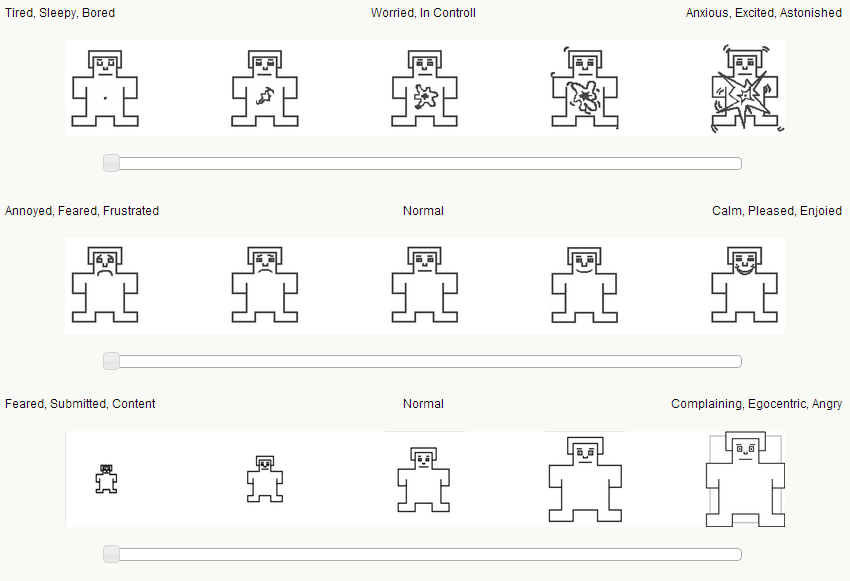
\includegraphics[width=0.7\textwidth]{images/sam.png}
  \label{fig:sam}
\end{figure}

\paragraph{Intrinsic Motivation Inventory}

Different components of game experience were measured using the Intrinsic Motivation Inventory questionnaire \cite{?}. It combines several game-related subjective measurement dimensions: interest/enjoyment, perceived competence, effort and felt pressure and tension while playing the game. Each one of these components consists of ?? question items (e.g., ``While playing, I was thinking about how much I enjoyed it'' is a interest/enjoyment component item). Question items were shown in a randomized order every time the page was viewed. Each question item consists of a statement on a five-point scale ranging from 1 (strongly disagreeing with the statement) to 5 (strongly agreeing with the statement). The questionnaire was developed based on survey studies \cite{?}.

\paragraph{Player Experience of Need Satisfaction}


\paragraph{Game Engagement Questionnaire}

%%%%%%%%%%%%%nasty%%%%%%%%%%%%%
An image of a regular participant signal values is depicted at
the following. In this image from left to right the light blue line
shows different conditions being played, and when the light blue
line is declining towards its base value, that is the period that
participant is asked to stop playing and instead relaxing and filling
out the questionnaires. The blue line is the normalized GSR signal
value of the participants which is used as an estimation of his
excitement level. The yellow green and pink lines are showing the
three different modes of Player, NPC and Environment parameters
being adapted

Following image is the GSR signal of players playing different
conditions from 1 to 4. From left to right the conditions are the
Default, Player, NPC and the Environment mode. This signals are all
based to an initial start value of 100, during the play experience,
some of them had gone bellow the start point and some other had risen
above that. Also the start time for each different condition is
shifted 500 seconds times the number of condition, from 0.

The following image is the average of GSR values for players in four
different conditions from left to right: Default, Player, NPC and
Environment modes
%%%%%%%%%%%%%nasty%%%%%%%%%%%%%

\section{Results}

% describe 16 participant's feedbacks and comments, and general ideas on how each one of them migh have experienced different situations through the game.

%-----------------------------------------------------------
\begin{center}
\label{tbl:players-stats}
\captionof{table}{Sixteen players with their performance, divided into four experience categories spread across all four conditions}
\begin{tabular}{+l^l^l^l^l}
\bhline
\rowstyle{\bfseries}
ID       &   Performance   &   Order   &   Experience   &   Condition \\
\hline
1        &   69            &   1       &   1            &   4 \\
2        &   74            &   1       &   2            &   1 \\
3        &   117           &   1       &   3            &   2 \\
4        &   106           &   1       &   4            &   3 \\
5        &   42            &   2       &   1            &   1 \\
6        &   86            &   2       &   2            &   2 \\
7        &   67            &   2       &   3            &   3 \\
8        &   118           &   2       &   4            &   4 \\
9        &   13            &   3       &   1            &   3 \\
10       &   106           &   3       &   2            &   4 \\
11       &   98            &   3       &   3            &   1 \\
12       &   140           &   3       &   4            &   2 \\
13       &   66            &   4       &   1            &   2 \\
14       &   58            &   4       &   2            &   3 \\
15       &   110           &   4       &   3            &   4 \\
16       &   140           &   4       &   4            &   1 \\
\bhline
\end{tabular}
\end{center}
%-----------------------------------------------------------

\img
{Normal Q-Q plot of players' performance}
{Normal Q-Q plot of players' performance}
{anova-qq-performance.pdf}
{players-qq-performance}

\img
{Plot of residuals vs. fitted values for players' performance}
{Plot of residuals vs. fitted values for players' performance}
{anova-residuals-vs-fitted-values-performance.pdf}
{residuals-vs-fitted-values-performance}


\img
{Normal Q-Q plot of players' excitement}
{Normal Q-Q plot of players' excitement}
{anova-qq-excitement.pdf}
{players-qq-excitement}

\img
{Plot of residuals vs. fitted values for players' excitement}
{Plot of residuals vs. fitted values for players' excitement}
{anova-residuals-vs-fitted-values-excitement.pdf}
{residuals-vs-fitted-values-excitement}

%-----------------------------------------------------------
\begin{center}
\label{tbl:unknown}
\captionof{table}{unknown}
\begin{tabular}{+l^l^l^l}
\bhline
\rowstyle{\bfseries}
Condition    & Mean estimation of performance   & Lower bound   & Upper bound \\
\hline
1            & 58.50                            &   45.60997    &   71.39003  \\
2            & 98.25                            &   85.35997    &   111.14003 \\
3            & 101.75                           &   88.85997    &   114.64003 \\
4            & 91.50                            &   78.60997    &   104.39003 \\
\bhline
\end{tabular}
\end{center}
%-----------------------------------------------------------

%%nasty from mahdi
In the above table we see that not all the means of performances of players across the conditions are equal. We use ANOVA to test whether the means are statistically equal. The p-value corresponding the hypothesis that all the means are equal is  0.01719944. Hence we come to realize that, at the level of 5\%, not all the means are equal. This may mean that manipulating the games may have changed the performances of the players. To see whether this assumption is true, we use Tukey's multiple comparison test. The results are as following:
%%nasty from mahdi

%-----------------------------------------------------------
\begin{center}
\label{tbl:unknown}
\captionof{table}{unknown}
\begin{tabular}{+l^l^l^l^l}
\bhline
\rowstyle{\bfseries}
Conditions' difference   &   Mean difference   &   Lower bound   &   Upper bound   &   P-value     \\
\hline
2-1                      &   39.75             &   10.787245     &   68.71276      &   0.0124504   \\
3-1                      &   43.25             &   14.287245     &   72.21276      &   0.0082819   \\
4-1                      &   33.00             &   4.037245      &   61.96276      &   0.0290272   \\
3-2                      &   3.50              &   -25.462755    &   32.46276      &   0.9732678   \\
4-2                      &   -6.75             &   -35.712755    &   22.21276      &   0.8492682   \\
4-3                      &   -10.25            &   -39.212755    &   18.71276      &   0.6351259   \\
\bhline
\end{tabular}
\end{center}
%-----------------------------------------------------------

% nasty from mahdi
The first three rows of the above table state that the players have significantly lower performance in the default condition, while the performances increase in the other three condition. The lower three rows of the table state that all the three conditions have the same influence on the default such that the performers have similar performances.

In this experiment, as mentioned earlier, we used Latin Square method. The blockings were Individuals' experiences and time order which were suspected to be nuisiance factors of this experiment. After apply the method, we gained the values:
F-ratio of run order= 1.2083 
F-ratio of experience= 29.0333.
The first value is small while the other is extremely large. We conclude that blocking the time order is not appropriate for such studies while experience had the potential to affect our results. In addition, we can say that different individuals' experiences resulted in different performances. This becomes more apparent when we note that if a player is more experienced than the other, s/he would have a better performance if the game is manipulated in order to make the game, sometimes, more challenging (condition 3) and sometimes of favour of the player (condition 2). The table below explains which condition is more suitable for different players with different game experiences:
% nasty from mahdi

%-----------------------------------------------------------
\begin{center}
\label{tbl:unknown}
\captionof{table}{unknown}
\begin{tabular}{+l^l^l^l^l}
\bhline
\rowstyle{\bfseries}
Experiences' difference   & Mean difference   & Lower bound   & Upper bound   & P-value     \\
\hline
2-1                       & 33.5              & 4.537245      & 62.46276      & 0.0271883   \\
3-1                       & 50.5              & 21.537245     & 79.46276      & 0.0037921   \\
4-1                       & 76.0              & 47.037245     & 104.96276     & 0.0004163   \\
3-2                       & 17.0              & -11.962755    & 45.96276      & 0.2745976   \\
4-2                       & 42.5              & 13.537245     & 71.46276      & 0.0090222   \\
4-3                       & 25.5              & -3.462755     & 54.46276      & 0.0812661   \\
\bhline
\end{tabular}
\end{center}
%-----------------------------------------------------------

%-----------------------------------------------------------
\begin{center}
\label{tbl:unknown}
\captionof{table}{unknown}
\begin{tabular}{+l^l^l^l}
\bhline
\rowstyle{\bfseries}
Condition     &   Mean of GSR   &   Lower bound   &   Upper bound   \\
\hline
Default       &   -5.29680      &   -24.13608     &   13.54248      \\
Player        &   46.48590      &   27.64662      &   65.32518      \\
Zombie        &   26.95377      &   8.11450       &   45.79305      \\
Environment   &   22.99617      &   4.15690       &   41.83545      \\
\bhline
\end{tabular}
\end{center}
%-----------------------------------------------------------

% nasty from mahdi
p-value of the hypothesis that the excitement of players were the same across all the conditions= 0.06439932.
the ration for experience is 2.230153 which is small. So experience doesn't have an influence on players' excitement.
% nasty from mahdi

\chapter{Discussion}                             \label{chap:discus}      %5 to 10 pages
%talk for the discussion
%State what you've done and what you've found
%Summarize contributions (achievements and impact)
%Outline open issues/directions for future work

The results of my design probe show that adapting the game resulted in higher arousal, but that not all methods were equally effective. In this section, I discuss how game developers and designers can apply my results, consider the limitations of my work, and present the opportunities for future research in this area.

\section{Applying the results}
My work suggests that adapting games based on a user's affective state can increase player arousal (excitement) and can potentially automate balancing the difficulty of the game with the affective state of the player. By increasing the challenge of the game when players are not aroused, I can personalize the game experience, drawing the player in. Conversely, by decreasing the challenge when players feel overwhelmed (too aroused), I can keep the game difficulty manageable and maintain player engagement.

My work aims to investigate how to adapt games based on a player's affective state – with the goal of keeping players optimally engaged with the system. Previous work has examined dynamic difficulty adjustment (DDA) for the purposes of balancing multiplayer game play (e.g., ~\cite{bateman2011target}). Previous research has shown that when multiplayer games are unbalanced (i.e., one player is much stronger than another), players do not have as much fun ~\cite{vicencio2014effectiveness}, and thus there is a need to provide assistance to one player (or hindrance to another) to better balance play. Different approaches have been used to adjust difficulty for player balancing (see ~\cite{bateman2011target} and ~\cite{vicencio2014effectiveness}); however, research has not systematically examined whether adjusting the abilities of the player, enemy, or environment affects game enjoyment or player perception. My work suggests that these different approaches change player experience and thus there is an opportunity to extend my work into the domain of DDA for balancing multiplayer games.

\section{Why adapting the NPC enemy reduced enjoyment}
My results suggest that helping the player or changing the environment to better support the player are better adaptation approaches than adapting the strength of the NPC enemies. Although a common approach in many games, reducing the difficulty by making the enemies easier to beat resulted in fewer zombie kills (as there were fewer zombies available to kill). This reduction in challenge may have resulted in lower ratings of perceived competence, which in turn reduced players' enjoyment in the NPC condition.

Self-determination theory ~\cite{ryan2000self} suggests that I strive to master challenges, and that this mastery over challenges creates a perception of competence – which is one of my basic needs that must be satisfied for well-being (along with the need for autonomy and need for relatedness). In the context of games, mastering challenges leads to competence, which ultimately leads to game enjoyment ~\cite{ryan2006motivational}. By adapting the NPC enemies, I give the player less of an opportunity to conquer a challenge, and thus less opportunity to experience competence (and as a result enjoyment). This approach thwarts players from satisfying their needs. Conversely, giving the player enhanced abilities or adapting the environment to support the player in their quest does not seem to negatively affect perceived competence. Adapting the spawn rate or value of helpful items (such as the grenade in my Player condition or the health pack in my Environment condition) does not seem to reduce experienced competence, but allows players to feel like they are achieving in the context of the game.

Recent research in violent imagery in games and the resulting aggression that players experience has suggested that impeding competence in video games fosters aggressive thoughts, regardless of the presence or absence of violent imagery ~\cite{przybylski2013competence}. The authors show how manipulating competence (through manipulating frustrating and complex control schemes, levels of player experience, or game challenges) thwarts need satisfaction amongst players, and increases their access to aggressive thoughts. Although the domain of evaluation (aggressive thoughts) is distinct from my goals, the hypothesis that impeding competence in games thwarts satisfaction of this basic need helps to explain why giving players less challenge to master (as in the NPC condition) does not work as well as giving players the tools and support needed to master greater challenges, as in the Player and Environment conditions.

\section{Limitations and future work}
This design probe represents preliminary work into the domain of affectively-adapting games. There are several limitations in my work that present opportunities for future research. First, the number of participants that I included in my design probe is low ($n=16$). Conducting a large-scale experiment would increase the power of my experiment and could reveal differences between the approaches or strengthen existing differences (e.g., the planned contrasts). Second, I investigated the adaptation in a single game genre (FPS game) with specific approaches (e.g., manipulating speed and weapons). Investigating whether my results hold in a different genre or with different adaptation choices would help to generalize my findings. Third, I only adapted based on a player's galvanic skin response. Employing the full affective engine to access arousal and valence (e.g., ~\cite{mandryk2007fuzzy}) would qualify the player's arousal as either positive or negative in nature. Finally, as noted previously in the discussion, I could consider applying my approach of adaptation based on performance variables, rather than player affect, to examine DDA for the purpose of balancing multiplayer games.


%------------------------------------------------------------------------------

% Bibliography
\uofsbibliography[plain]{content/bibliography}

%------------------------------------------------------------------------------

% APPENDICES
\uofsappendix
\chapter{Transforming physiological variables into arousal-valence space} \label{app:phys-to-av}    
The following 22 rules were used as described in Section ~\ref{subsec:fuzzi} to transform physiological variables into arousal-valence space:

\begin{lstlisting}[language=python]
if (GSR      is high     )                        then (arousal is high     )
if (GSR      is mid-high )                        then (arousal is mid-high )
if (GSR      is mid-low  )                        then (arousal is mid-low  )
if (GSR      is low      )                        then (arousal is low      )
if (HR       is low      )                        then (arousal is low      )
if (HR       is high     )                        then (arousal is high     )
if (EMGfrown is high     )                        then (valence is very low )
if (EMGfrown is mid      )                        then (valence is low      )
if (EMGsmile is mid      )                        then (valence is high     )
if (EMGsmile is high     )                        then (valence is very high)
if (GSR      is low      ) and (HR is high)       then (arousal is midlow   )
if (GSR      is high     ) and (HR is low )       then (arousal is midhigh  )
if (GSR      is high     ) and (HR is mid )       then (arousal is high     )
if (GSR      is mid-high ) and (HR is mid )       then (arousal is mid-high )
if (GSR      is mid-low  ) and (HR is mid )       then (arousal is mid-low  )
if (EMGsmile is low      ) and (EMGfrown is low ) then (valence is neutral  )
if (EMGsmile is high     ) and (EMGfrown is low ) then (valence is very high)
if (EMGsmile is high     ) and (EMGfrown is mid ) then (valence is high     )
if (EMGsmile is low      ) and (EMGfrown is high) then (valence is very low )
if (EMGsmile is mid      ) and (EMGfrown is high) then (valence is low      )
if (EMGsmile is low      ) and (EMGfrown is low ) and (HR is low)  then (valence is low)
if (EMGsmile is low      ) and (EMGfrown is low ) and (HR is high) then (valence is high)
\end{lstlisting}

\chapter{Transforming physiological variables into arousal-valence space} \label{app:phys-to-av}    
The following 22 rules were used as described in Section ~\ref{subsec:fuzzi} to transform physiological variables into arousal-valence space:

\begin{lstlisting}[language=python]
if (GSR      is high     )                        then (arousal is high     )
if (GSR      is mid-high )                        then (arousal is mid-high )
if (GSR      is mid-low  )                        then (arousal is mid-low  )
if (GSR      is low      )                        then (arousal is low      )
if (HR       is low      )                        then (arousal is low      )
if (HR       is high     )                        then (arousal is high     )
if (EMGfrown is high     )                        then (valence is very low )
if (EMGfrown is mid      )                        then (valence is low      )
if (EMGsmile is mid      )                        then (valence is high     )
if (EMGsmile is high     )                        then (valence is very high)
if (GSR      is low      ) and (HR is high)       then (arousal is midlow   )
if (GSR      is high     ) and (HR is low )       then (arousal is midhigh  )
if (GSR      is high     ) and (HR is mid )       then (arousal is high     )
if (GSR      is mid-high ) and (HR is mid )       then (arousal is mid-high )
if (GSR      is mid-low  ) and (HR is mid )       then (arousal is mid-low  )
if (EMGsmile is low      ) and (EMGfrown is low ) then (valence is neutral  )
if (EMGsmile is high     ) and (EMGfrown is low ) then (valence is very high)
if (EMGsmile is high     ) and (EMGfrown is mid ) then (valence is high     )
if (EMGsmile is low      ) and (EMGfrown is high) then (valence is very low )
if (EMGsmile is mid      ) and (EMGfrown is high) then (valence is low      )
if (EMGsmile is low      ) and (EMGfrown is low ) and (HR is low)  then (valence is low)
if (EMGsmile is low      ) and (EMGfrown is low ) and (HR is high) then (valence is high)
\end{lstlisting}

\chapter{Transforming arousal-valence space into emotional states}        \label{app:av-to-emotion} 
The following 67 rules were used as described in Section ~\ref{subsec:fuzzi} to convert arousal and valence into boredom, challenge, excitement, frustration, and fun:

\begin{enumerate}
\item If (arousal is not veryLow) and (valence is midHigh) then (fun is low)
\item If (arousal is not low) and (valence is midHigh) then (fun is low)
\item If (arousal is not veryLow) and (valence is high) then (fun is medium)
\item If (valence is veryHigh) then (fun is high)
\item If (arousal is midHigh) and (valence is midLow) then (challenge is low)
\item If (arousal is midHigh) and (valence is midHigh) then (challenge is low)
\item If (arousal is high) and (valence is midLow) then (challenge is medium)
\item If (arousal is high) and (valence is midHigh) then (challenge is medium)
\item If (arousal is veryHigh) and (valence is midLow) then (challenge is high)
\item If (arousal is veryHigh) and (valence is midHigh) then (challenge is high)
\item If (arousal is midLow) and (valence is midLow) then (boredom is low)
\item If (arousal is midLow) and (valence is low) then (boredom is medium)
\item If (arousal is low) and (valence is low) then (boredom is medium)
\item If (arousal is low) and (valence is midLow) then (boredom is medium)
\item If (arousal is midLow) and (valence is veryLow) then (boredom is high)
\item If (arousal is low) and (valence is veryLow) then (boredom is high)
\item If (arousal is veryLow) and (valence is veryLow) then (boredom is high)
\item If (arousal is veryLow) and (valence is low) then (boredom is high)
\item If (arousal is veryLow) and (valence is midLow) then (boredom is high)
\item If (arousal is midHigh) and (valence is midLow) then (frustration is low)
\item If (arousal is midHigh) and (valence is low) then (frustration is medium)
\item If (arousal is high) and (valence is low) then (frustration is medium)
\item If (arousal is high) and (valence is midLow) then (frustration is medium)
\item If (arousal is midHigh) and (valence is veryLow) then (frustration is high)
\item If (arousal is high) and (valence is veryLow) then (frustration is high)
\item If (arousal is veryHigh) and (valence is veryLow) then (frustration is high)
\item If (arousal is veryHigh) and (valence is low) then (frustration is high)
\item If (arousal is veryHigh) and (valence is midLow) then (frustration is high)
\item If (valence is veryLow) then (fun is veryLow)(challenge is veryLow)
\item If (valence is low) then (fun is veryLow)(challenge is veryLow)
\item If (valence is high) then (challenge is veryLow)(boredom is veryLow)(frustration is veryLow)
\item If (valence is veryHigh) then (challenge is veryLow) (boredom is veryLow)(frustration is veryLow)
\item If (valence is midHigh) then (boredom is veryLow) (frustration is veryLow)
\item If (arousal is veryLow) then (challenge is veryLow) (frustration is veryLow)
\item If (arousal is low) then (challenge is veryLow)(frustration is veryLow)
\item If (arousal is midLow) then (challenge is veryLow) (frustration is veryLow)
\item If (arousal is midHigh) then (boredom is veryLow)
\item If (arousal is high) then (boredom is veryLow)
\item If (arousal is veryHigh) then (boredom is veryLow)
\item If (arousal is veryLow) and (valence is midHigh) then (fun is veryLow)
\item If (arousal is low) and (valence is midHigh) then (fun is veryLow)
\item If (arousal is veryLow) and (valence is high) then (fun is low)
\item If (valence is midLow) then (fun is veryLow)
\item If (arousal is veryLow) and (valence is high) then (boredom is low)
\item If (arousal is low) and (valence is midHigh) then (boredom is low)
\item If (arousal is veryLow) and (valence is midHigh) then (boredom is medium)
\item If (arousal is veryHigh) and (valence is veryLow) then (challenge is medium)
\item If (arousal is veryHigh) and (valence is veryHigh) then (challenge is medium)
\item If (arousal is high) and (valence is low) then (challenge is low)
\item If (arousal is high) and (valence is high) then (challenge is low)
\item If (arousal is veryHigh) and (valence is low) then (challenge is high)
\item If (arousal is veryHigh) and (valence is high) then (challenge is high)
\item If (arousal is midHigh) and (valence is midHigh) then (excitement is low)
\item If (arousal is high) and (valence is midHigh) then (excitement is medium)
\item If (arousal is high) and (valence is high) then (excitement is medium)
\item If (arousal is midHigh) and (valence is high) then (excitement is medium)
\item If (arousal is veryHigh) and (valence is midHigh) then (excitement is high)
\item If (arousal is veryHigh) and (valence is high) then (excitement is high)
\item If (arousal is veryHigh) and (valence is veryHigh) then (excitement is high)
\item If (arousal is high) and (valence is veryHigh) then (excitement is high)
\item If (arousal is midHigh) and (valence is veryHigh) then (excitement is high)
\item If (arousal is midLow) then (excitement is veryLow)
\item If (arousal is low) then (excitement is veryLow)
\item If (arousal is veryLow) then (excitement is veryLow)
\item If (valence is veryLow) then (excitement is veryLow)
\item If (valence is low) then (excitement is veryLow)
\item If (valence is midLow) then (excitement is veryLow)
\end{enumerate}

\chapter{Consent Form}                                                    \label{app:consent}       \addtolength{\wpYoffset}{-1.6cm}\ThisCenterWallPaper{0.85}{content/app-consent-form.pdf}
\chapter{Demographics Questionnaire}                                      \label{app:q-dmg}         \noindent\makebox[\textwidth][c]{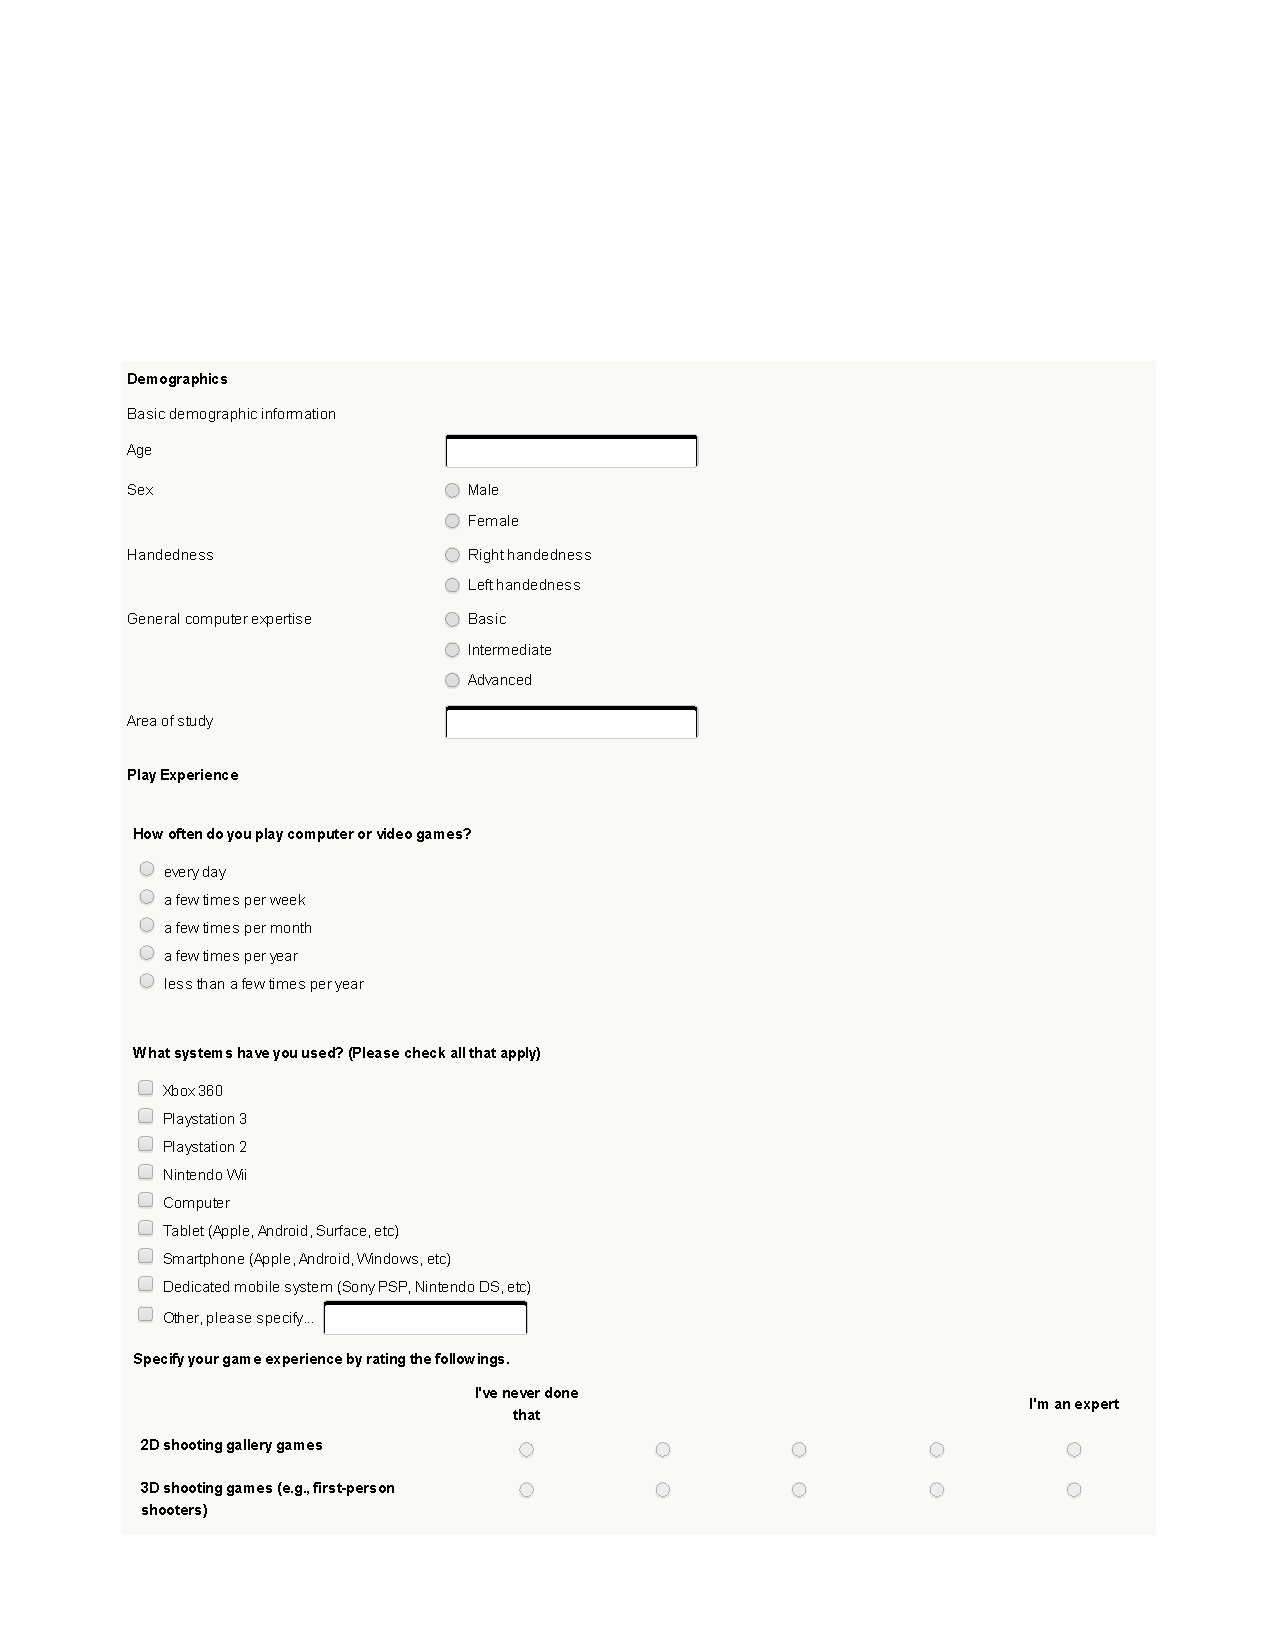
\includegraphics[page=1,width=\textwidth,height=\textheight,keepaspectratio]{content/app-q-dmg.pdf}}\newpage
                                                                                                    \noindent\makebox[\textwidth][c]{\includegraphics[page=2,width=\textwidth,height=\textheight,keepaspectratio]{content/app-q-dmg.pdf}}\newpage
                                                                                                    \noindent\makebox[\textwidth][c]{\includegraphics[page=3,width=\textwidth,height=\textheight,keepaspectratio]{content/app-q-dmg.pdf}}
\chapter{Condition Questionnaire}                                         \label{app:q-cnd}         \noindent\makebox[\textwidth][c]{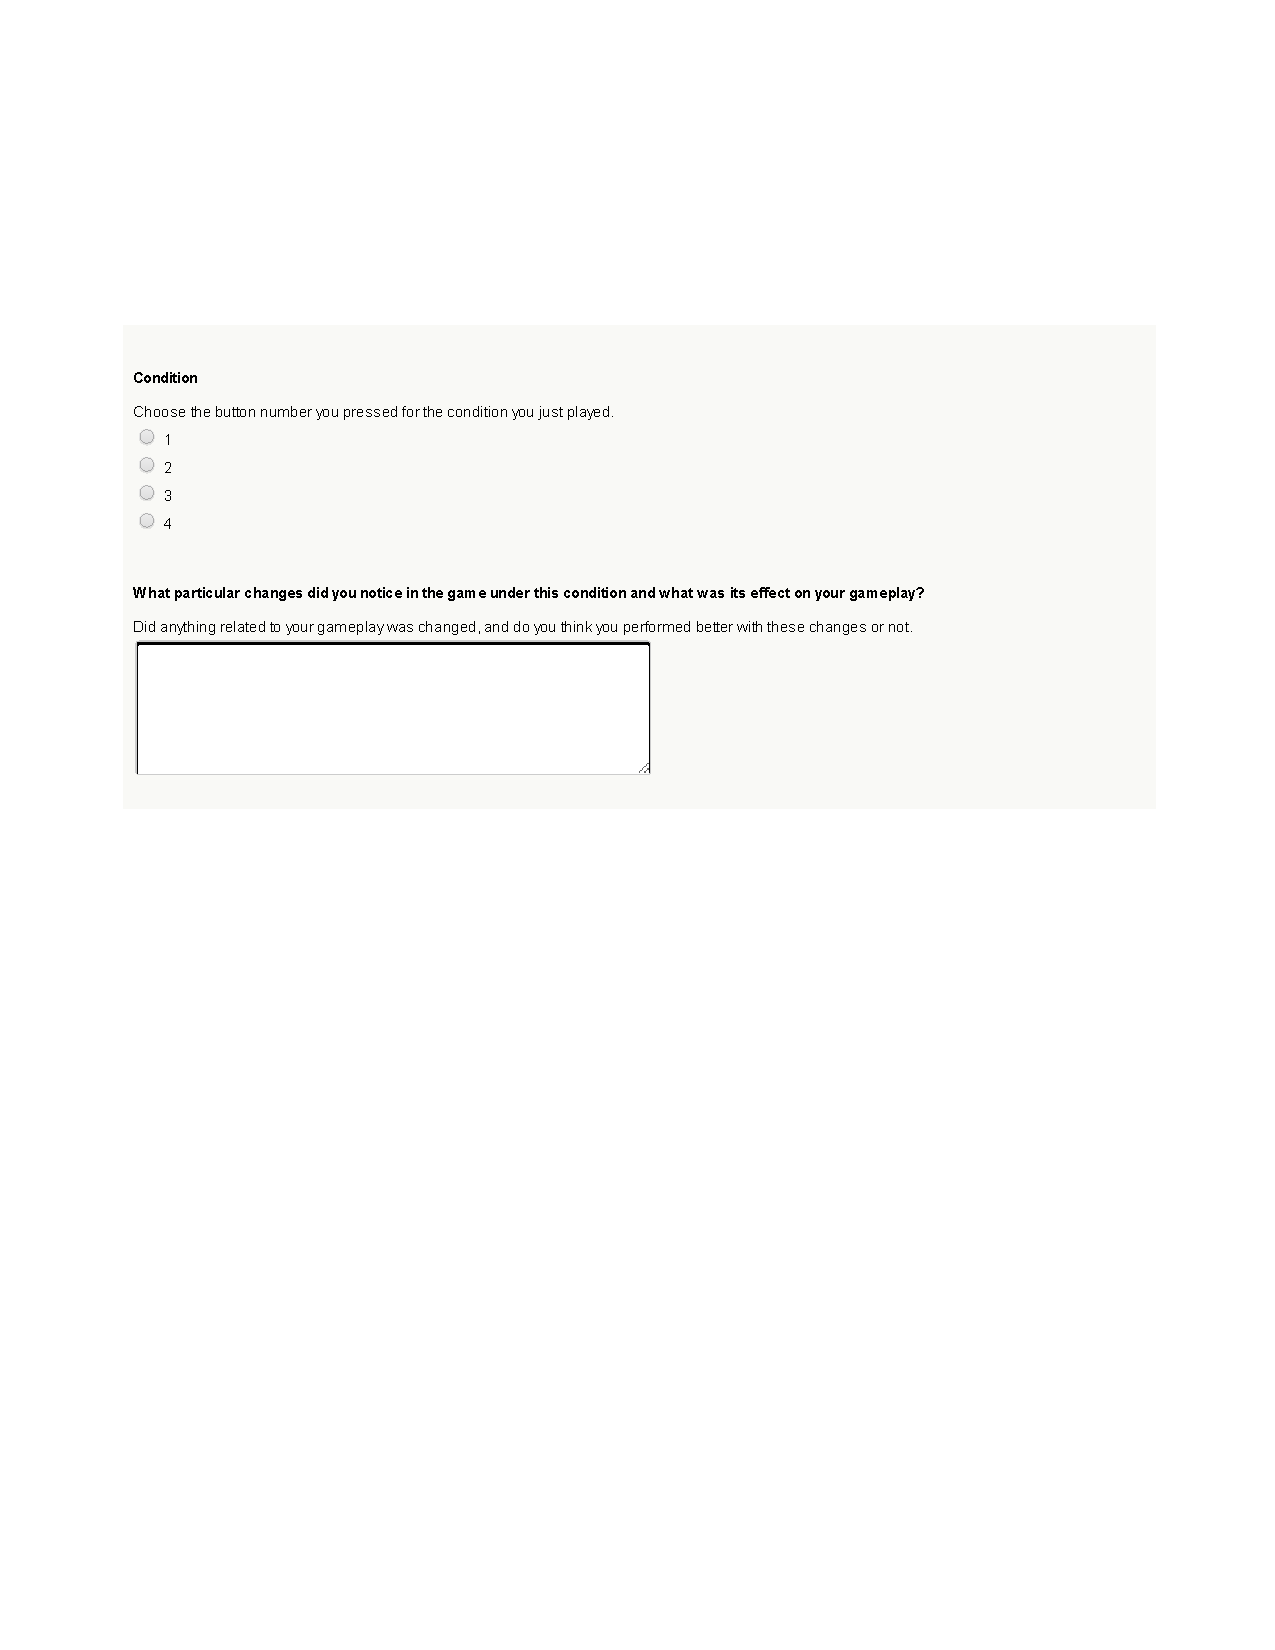
\includegraphics[width=\textwidth,height=\textheight,keepaspectratio]{content/app-q-cnd.pdf}}
\chapter{Self-Assessment-Manikin Arousal Scales Questionnaire}            \label{app:q-sam}         \noindent\makebox[\textwidth][c]{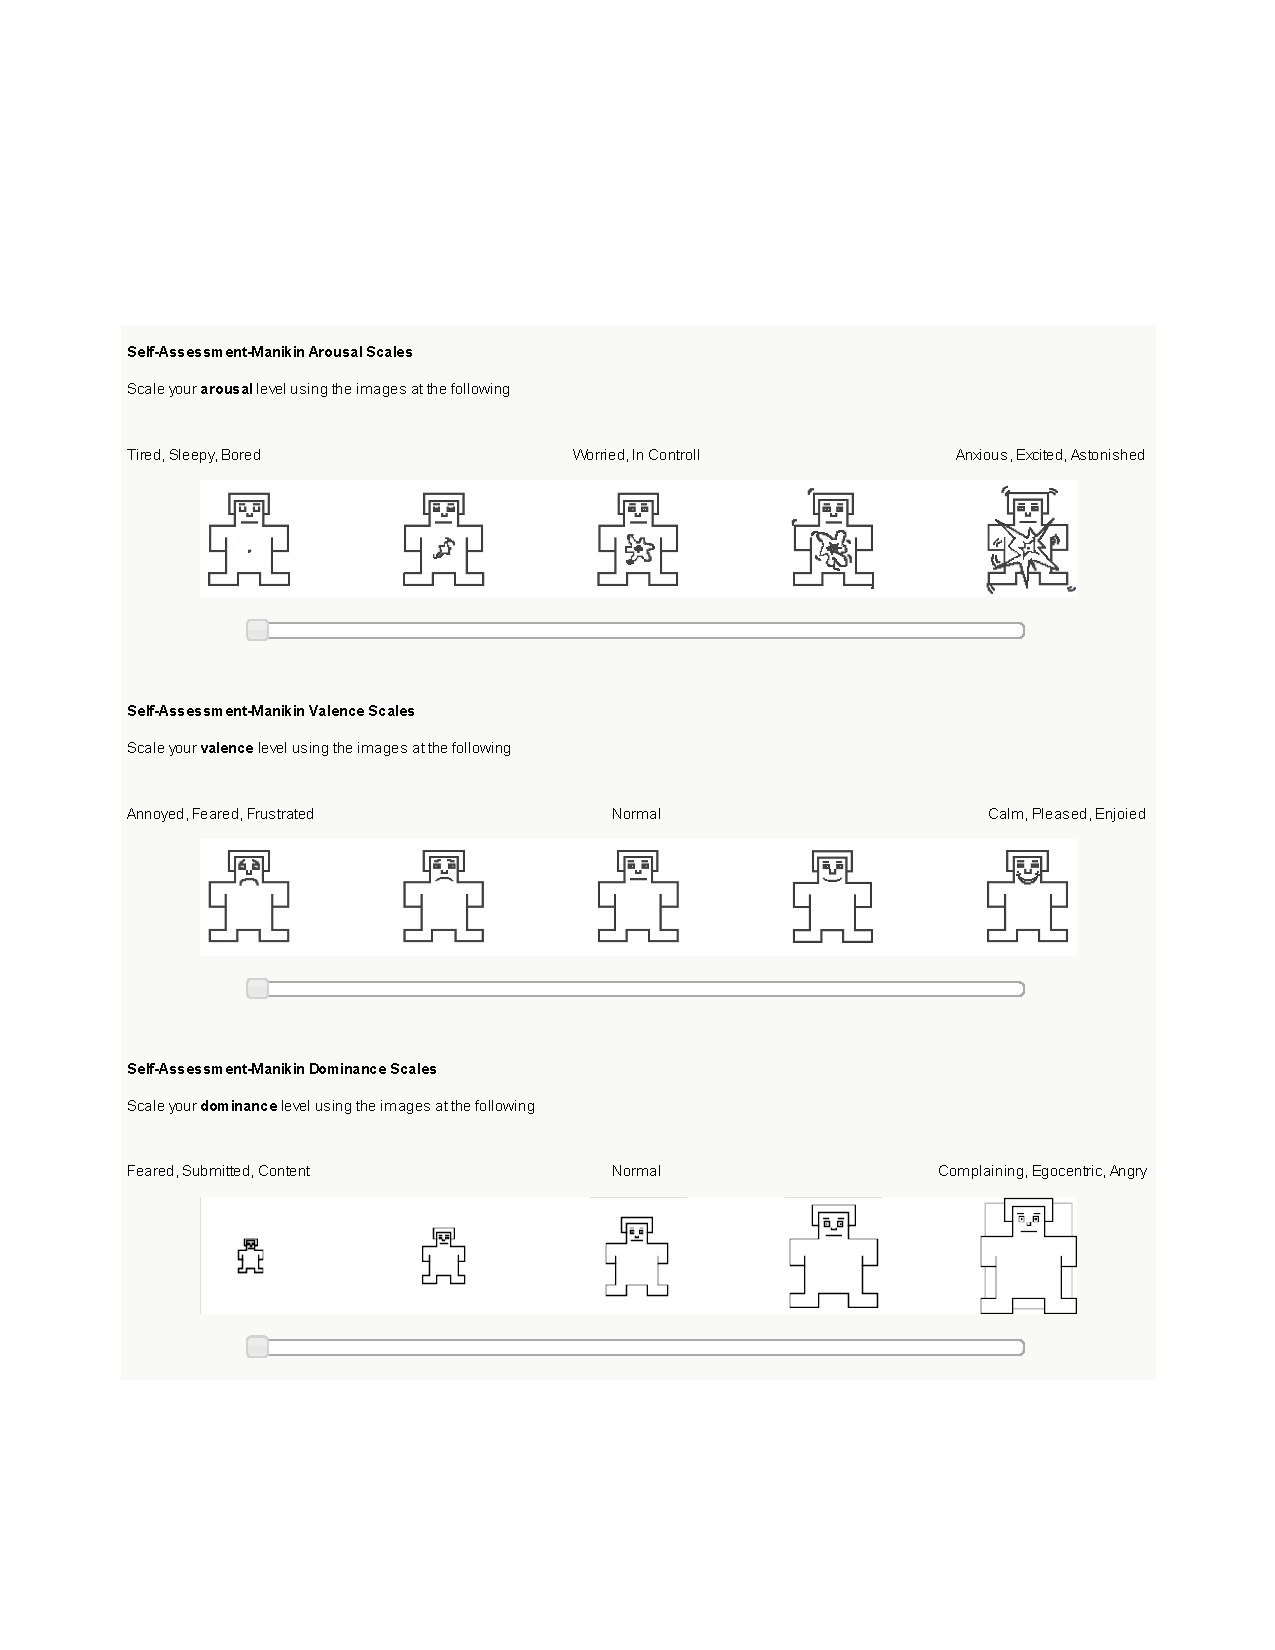
\includegraphics[width=\textwidth,height=\textheight,keepaspectratio]{content/app-q-sam.pdf}}
\chapter{Intrinsic Motivation Inventory Questionnaire}                    \label{app:q-ini}         \noindent\makebox[\textwidth][c]{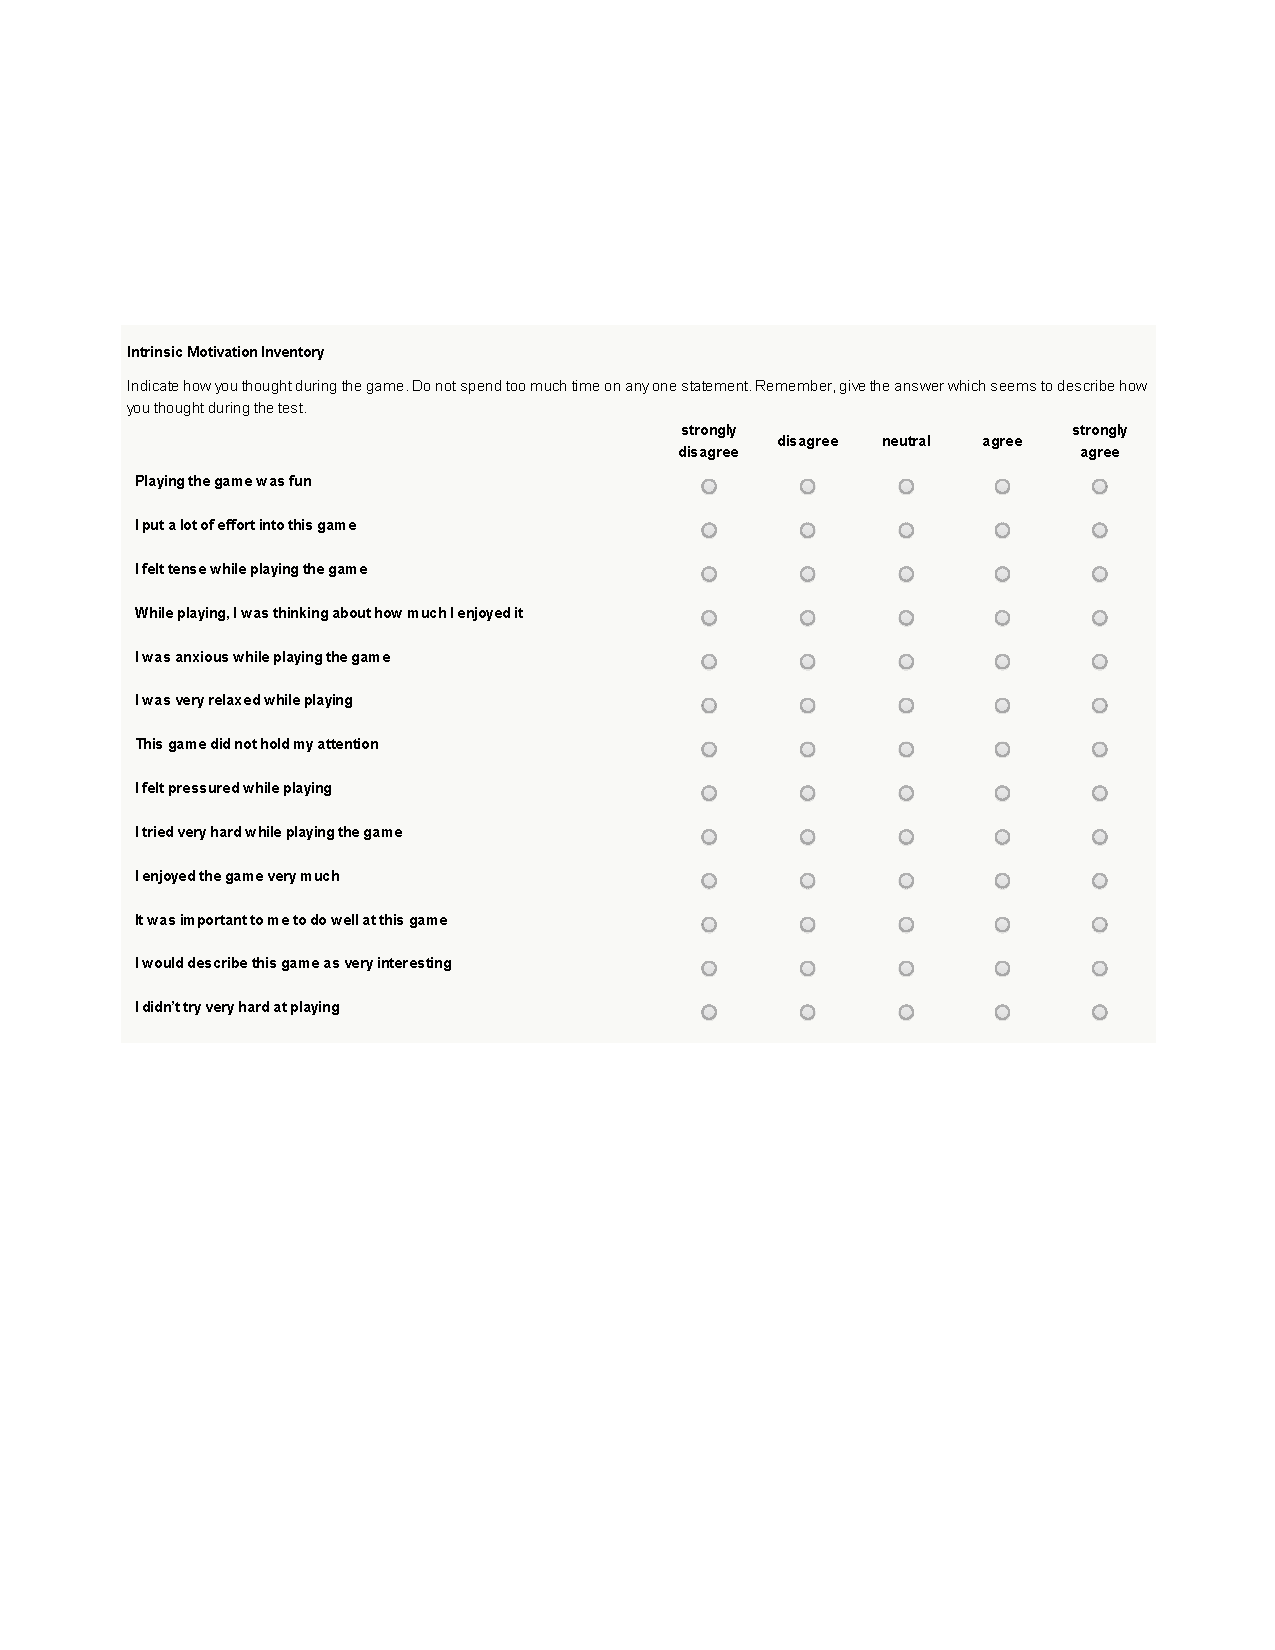
\includegraphics[width=\textwidth,height=\textheight,keepaspectratio]{content/app-q-imi.pdf}}
\chapter{Player Experience of Need Satisfaction Questionnaire}            \label{app:q-pens}        \noindent\makebox[\textwidth][c]{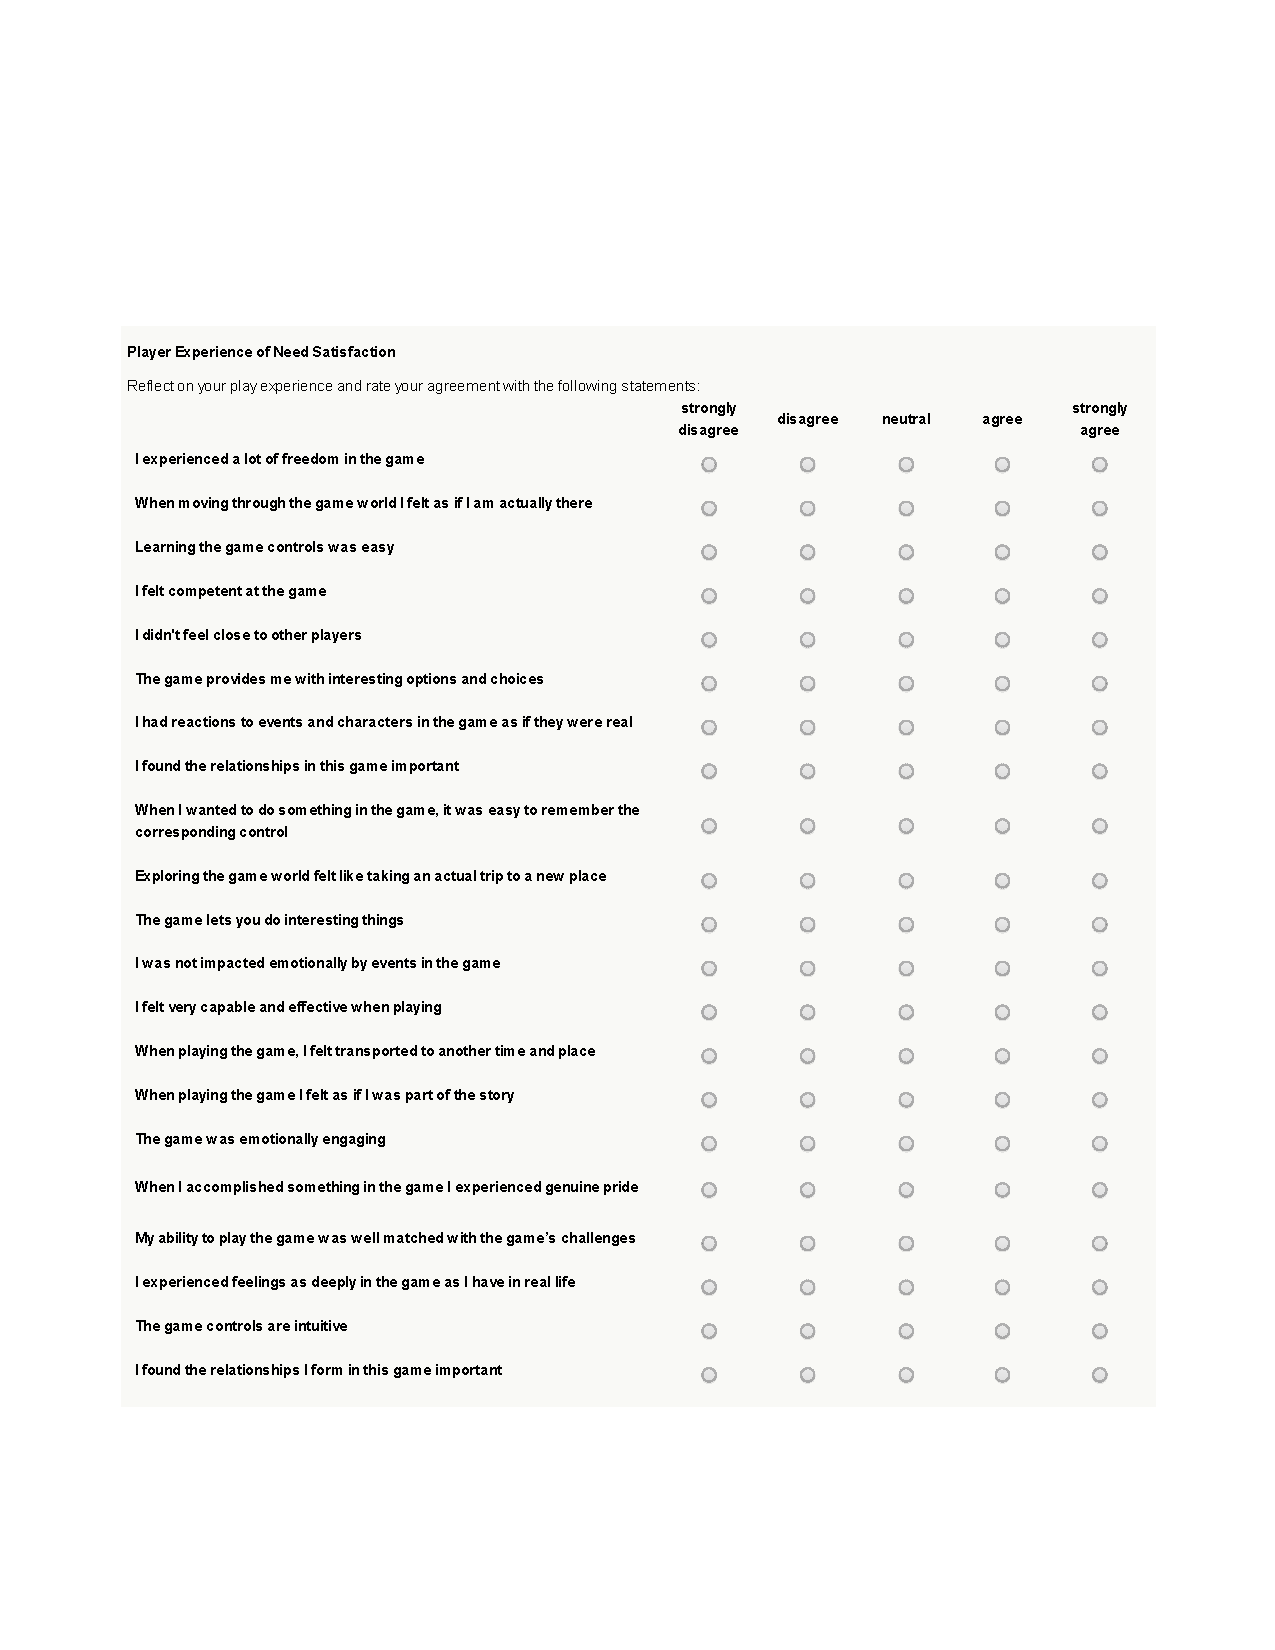
\includegraphics[width=\textwidth,height=\textheight,keepaspectratio]{content/app-q-pens.pdf}}
\chapter{Game Engagement Questionnaire}                                   \label{app:q-geq}         \noindent\makebox[\textwidth][c]{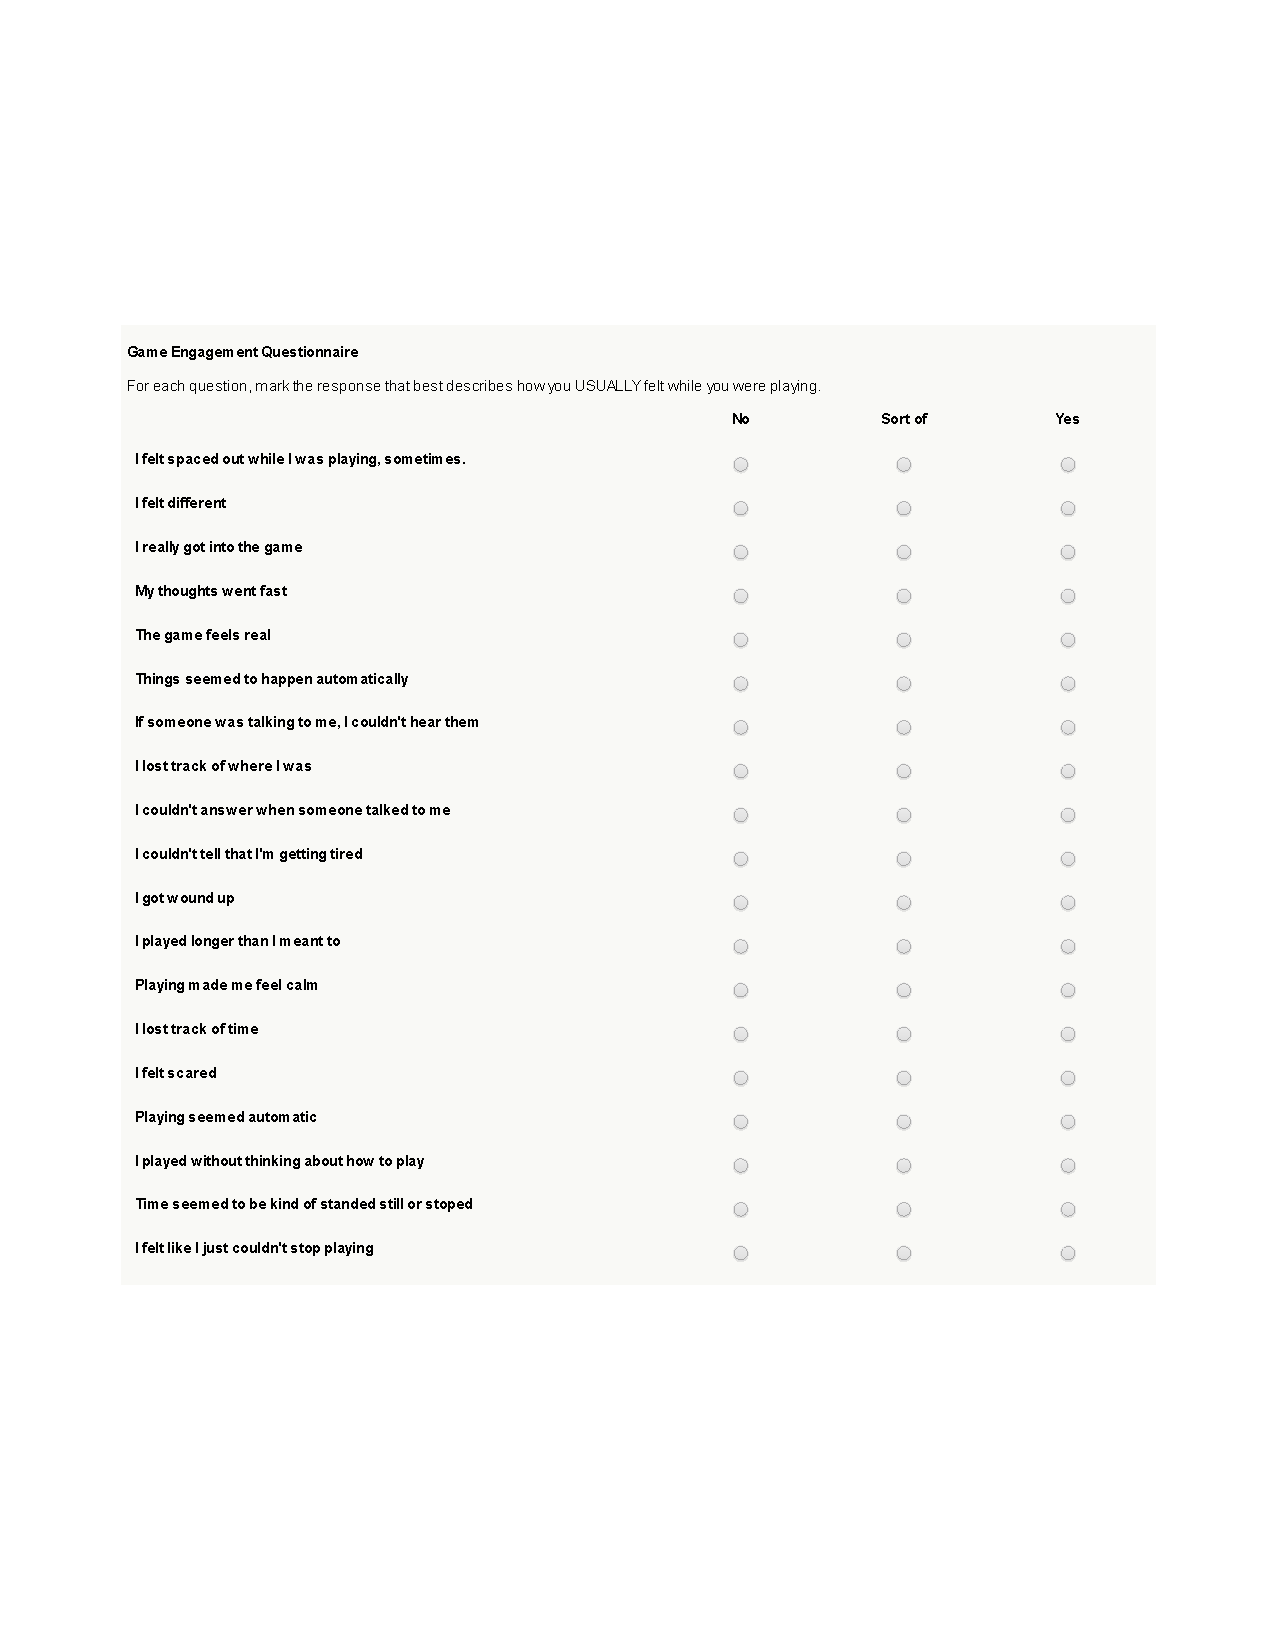
\includegraphics[width=\textwidth,height=\textheight,keepaspectratio]{content/app-q-geq.pdf}}

%------------------------------------------------------------------------------

\end{document}

%------------------------------------------------------------------------------
